% \chapter{Methods and data}

\chapter{Modelling renewable energy technologies}
\label{methods_physical}

\vspace{-15pt} % -15pts for two-line heading, -45pts for single-line heading
\begin{tcolorbox}[enhanced,width=\textwidth,size=fbox,
        sharp corners,colframe=black!5!white,drop fuzzy shadow southeast,
        boxrule=3mm, parbox=false] 
        
This chapter borrows from the articles \citep{walch_big_2020,walch_quantifying_2021}:

\qquad \bibentry{walch_big_2020}

\qquad \bibentry{walch_quantifying_2021}
\end{tcolorbox}

Spatio-temporal modelling of renewable energy potentials integrates physical models of the renewable resources and technologies with geospatial operations using Geographic Information Systems (GIS).
The present chapter introduces state-of-the-art modelling approaches for two types of renewables addressed in this thesis, namely rooftop solar energy (Section \ref{method_solar}) and shallow geothermal energy (Section \ref{geo_method}). 
\nomenclature[A]{GIS}{Geographic Information Systems}
Relevant physical, geographical and technical constraints for both energy resources are outlined and popular modelling approaches are summarized, such as to justify the methods used in the large-scale estimation of rooftop solar potential (Chapter \ref{solar}) and shallow geothermal potential (Chapter \ref{geothermal}).

\section{Rooftop solar energy}
\label{method_solar}
\label{method_solar_hierarchy}
% and solar thermal 

Rooftop solar energy is defined here as the electrical or thermal energy harvested from installations on building rooftops, using solar photovoltaic (PV) panels or solar thermal collectors (STC), respectively. 
While we focus on the estimation of solar photovoltaic (PV) potential, which is currently the most frequently deployed solar technology on rooftops \cite{kaufmann_schweizerische_2017}, most parts of the methodology (except the techological model of the solar PV panels) are transferable to STC. 
\nomenclature[A]{STC}{Solar thermal collector}
\nomenclature[A]{RPV}{Rooftop photovoltaics}
This section reviews state-of-the-art approaches to model the hourly energy yield of rooftop-mounted solar PV systems in the context of large-scale potential studies, and justifies the choice of the empirical models (Section~\ref{phys_models}), geospatial techniques (Section~\ref{GIS_methods}) and the modelling approach for PV panels on flat roofs (Section~\ref{app_flat}) used in the large-scale rooftop PV potential estimation presented in Chapter~\ref{solar}. We hereby do not claim to provide a complete review of existing modelling approaches, but rather give an overview of the relevant modelling steps and outline popular computational methods for each step.

\begin{figure}[tb]
	\centering
	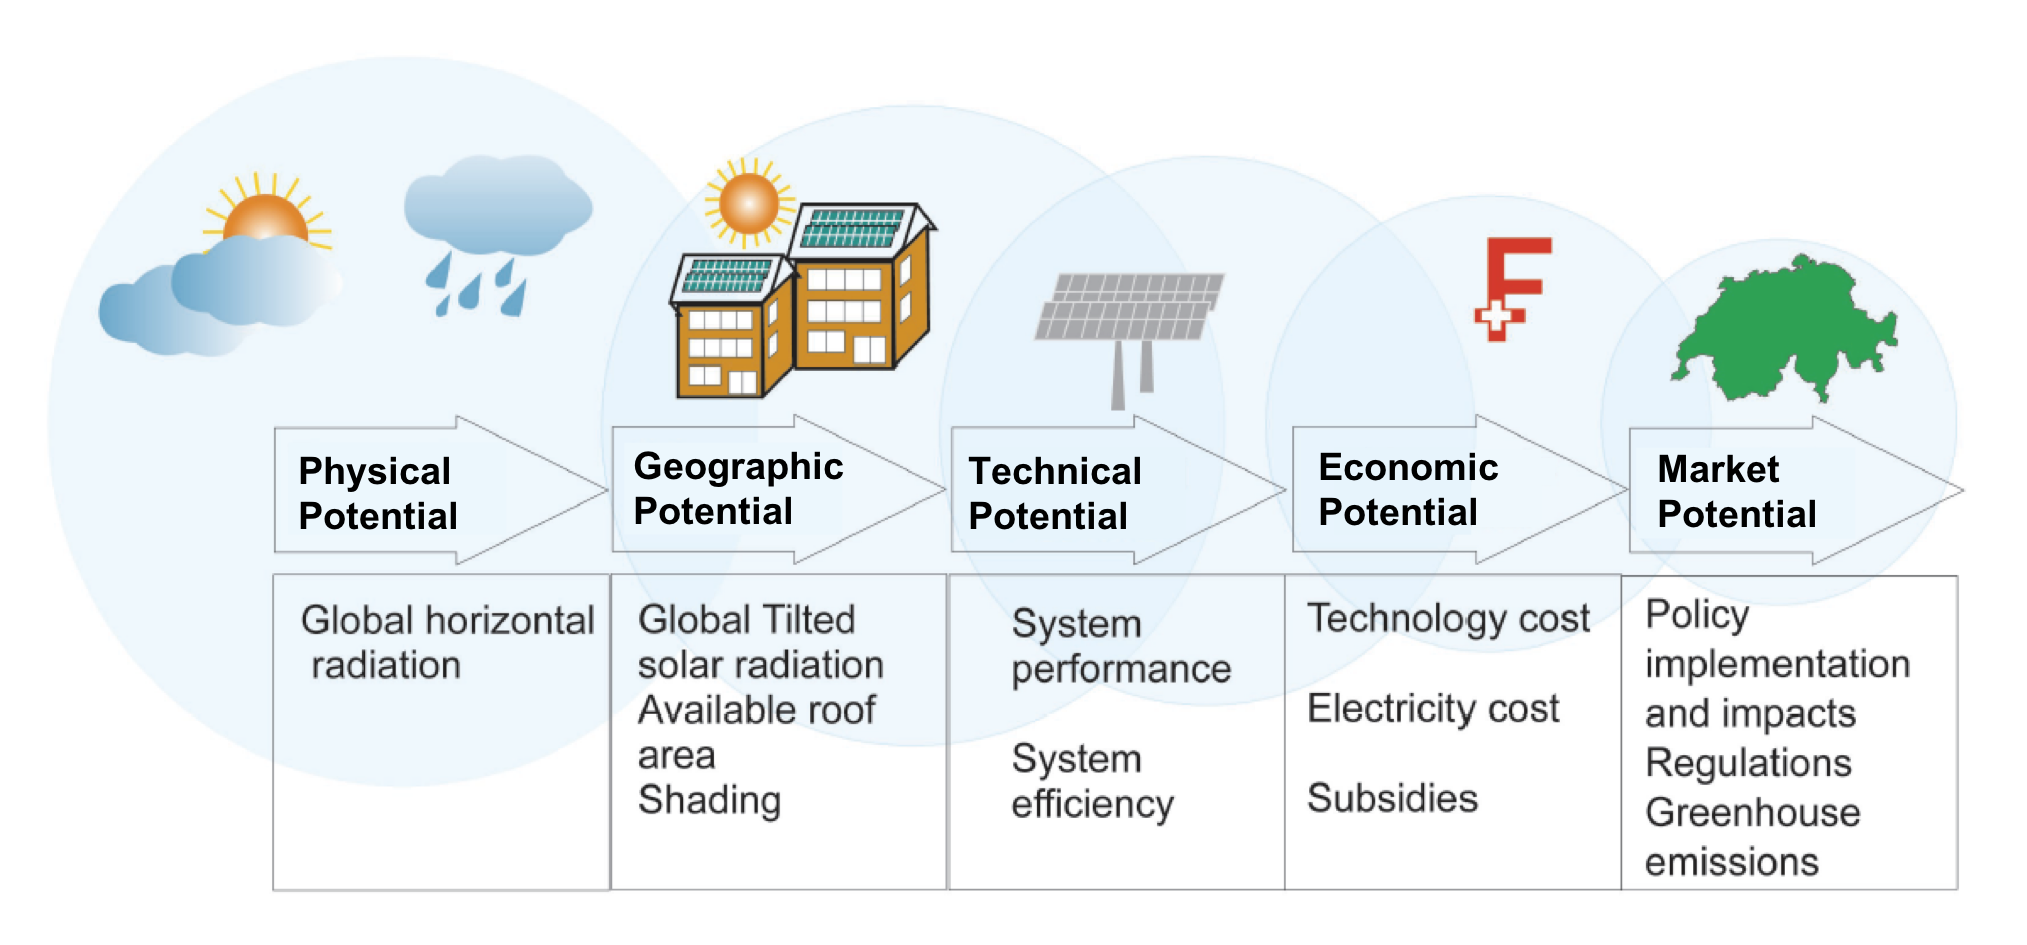
\includegraphics[width=\linewidth]{images/Figs/hierarchy.png}  
	\caption{Hierarchical approach for estimating rooftop PV potential. Source: \citet{assouline_estimation_2017}}
	\label{fig:solar_hierarchy}
\end{figure}

% SOURCE: CISBAT comparison paper
To compute the technical rooftop PV potential,  a hierarchical approach, shown in Fig.~\ref{fig:solar_hierarchy}, has been widely accepted in the literature \cite{assouline_quantifying_2017,ramirez_camargo_spatio-temporal_2015,izquierdo_method_2008,wiginton_quantifying_2010}. It includes (i) \textit{physical potential}, that is, the amount of solar energy reaching the earth’s surface, (ii) \textit{geographic potential}, that is, the amount of solar radiation received by the tilted PV panels, which is affected by the geometry of the panel (slope and aspect), the shading from surrounding buildings and trees and the suitable area for the panel installation, and (iii) \textit{technical potential}, that is, the maximum electricity output considering the technical characteristics of the PV technology (e.g. efficiency and system performance).

After obtaining the maximum feasible electricity output, one may consider additional environmental, economic or social considerations to refine the estimated size of the system. A fourth step may thus be an \textit{economic potential} focused on sizing the systems under given constraints. Economic considerations such as technology cost are not taken into account in most large-scale studies. Instead, these are typically assessed in separate studies that use the technical PV potential as input, in smaller-scale case studies as well as in hybrid potential assessments. An analysis of \textit{market potential} is beyond the scope of this work. 

\textbf{Physical potential.} The incoming solar radiation (also referred to as irradiance, in W/m$^2$), consists of three compotents: (i) a direct or beam component ($G_B$), which describes the direct incoming solar radiation on a horizontal plane, (ii) a diffuse component ($G_D$), which is diffracted for example through the atmosphere and through cloud coverage, and (iii) a surface reflected component $G_R$, which is driven by the ground surface reflectance, also known as albedo ($\rho$), but which can be omitted for horizontal planes \cite{assouline_estimation_2017}. Omitting $G_R$, the global horizontal solar radiation $G_h$ is given by \cite{assouline_estimation_2017}:
\begin{equation}
\label{eq:Gh_method}
G_{h} = G_{B} + G_{D}
\end{equation}
While most large-scale studies of RPV potential use satellite data or station measurements to obtain $G_h, G_B, G_D$ (e.g. \cite{bodis_high-resolution_2019,buffat_scalable_2018,ramirez_camargo_spatio-temporal_2015,calcabrini_simplified_2019}), empirical models exist to derive these from related variables such as the sunshine duration and the extra-terrestrial solar radiation \cite{assouline_estimation_2017}. 
In other cases, (geo)-statistical methods have been developed to estimate solar radiation. 
These include averaging the nearest neighbours \cite{klauser_solarpotentialanalyse_2016}, geostatistical methods such as kriging \cite{alsamamra_comparative_2009,rehman_spatial_2000} as well as machine learning approaches such as Support Vector Machines \cite{assouline_quantifying_2017}, Random Forests \cite{assouline_large-scale_2018} and neural networks \cite{hocaoglu_hourly_2008,notton_neural_2013,sahin_application_2013}. As averaging tends to oversimplify the modelling, and kriging is computationally intensive and requires modelling of anisotropic spatial correlations and stationarity of the process, the data-driven machine learning algorithms have recently gained much attention due to their performance and speed \cite{kanevski_machine_2009}. 
Most models do not estimate the uncertainty related to modelling horizontal irradiance, which is an important aspect if the results are processed further.
A further review of different modelling techniques for horizontal solar radiation is provided in \cite{zhang_review_2018}.

\textbf{Geographic potential.} The solar power received by RPV panels is driven by two factors: (i) the incoming solar radiation on the tilted panels, and (ii) the available area for installing PV, sometimes also quantified as the number of panels that can be installed on a rooftop. As the global horizontal radiation, the tilted radiation ($G_t$) is composed of a direct ($G_{Bt}$), a diffuse ($G_{Dt}$) and a reflected ($G_{Rt}$) component, such that \cite{assouline_estimation_2017}:
\begin{equation}
\label{eq:POA}
G_{t} = G_{Bt} + G_{Dt} + G_{Rt}
\end{equation}

The three components in Eq.~\ref{eq:POA} describe the plane-of-array (POA) radiation, obtained from empirical models (Section~\ref{phys_models}), which represents the radiation received by a fully unshaded PV panel in an open space. 
In urban environments, however, direct shading and a reduced sky visibility from surrounding buildings or other built-up objects, referred to as the sky view factor (SVF), can significantly impact the electricity yield of a PV panel. 
Hence, many studies of rooftop PV potential use geospatial techniques based on 2D or 3D models of the urban environment, detailed in Section~\ref{GIS_methods}, to quantify shading effects and the SVF (e.g.~\cite{desthieux_solar_2018,calcabrini_simplified_2019,wegertseder_combining_2016,jakubiec_method_2013}).
As these are included across the literature in the form of different factors, partially due to different spatial and temporal resolutions of RPV studies, we do not provide a generalised formulation to include these factors in Eq.~\ref{eq:POA}. However, in Chapter~\ref{solar_comparison} we will attempt to formulate such a generalisation for studies carried out in Switzerland.

The available area for installing PV or STC ($A_{PV}$) is potentially the factor that varies most between different studies of RPV potential, as it is strongly dependent on the scale of the study and on the available rooftop data. 
Rooftop available area is either quantified as constant factors (e.g. \cite{iea_potential_2002,wegertseder_combining_2016,portmann_sonnendach.ch:_2016}) or derived from building data (\cite{ramirez_camargo_spatio-temporal_2015,assouline_quantifying_2017,hong_development_2017}) and aerial imagery \cite{mainzer_assessment_2017} using geospatial techniques or image processing. 
As the required geospatial input data may not be available across entire study areas and the computational time for these methods may be prohibitively high, sampling techniques \cite{izquierdo_method_2008}, the use of building prototypes \cite{wegertseder_combining_2016} and extrapolation techniques using ML \cite{assouline_quantifying_2017,assouline_large-scale_2018} based on geospatial methods are frequently used in large-scale studies. 
A review of statistical and geospatial techniques for quantifying the available roof area is provided in Section~\ref{GIS_methods}, differentiating between the quantification of the total roof area, the useful roof area and the roof suitability for PV installations.

\textbf{Technical potential.} The conversion of global radiation to PV potentials is driven by three factors: the efficiency of the PV panel ($\eta_{PV}$), the inverter efficiency ($\eta_\mathit{inv}$) and other losses ($\eta_\mathit{losses}$), which are multiplied with the tilted radiation ($G_t$) and the available area for PV installation ($A_{PV}$):
\begin{equation}
    P_{PV} = G_t \times A_{PV} \times \eta_{PV} \times \eta_\mathit{inv} \times \eta_\mathit{losses}
\end{equation}
While several studies use constant values for panel and inverter efficiencies \cite{assouline_quantifying_2017,wegertseder_combining_2016,romero_rodriguez_assessment_2017,ordonez_analysis_2010,hong_development_2017}, many high-resolution PV potential studies use analytical or empirical models to quantify the efficiencies as a function of radiation, temperature, wind speed and technical characteristics of PV systems. The level of detail of these models ranges from the analytical modelling of invidual cells and their arrangement in a PV panel \cite{buffat_scalable_2018} to entirely coefficient-based empirical models \cite{mainzer_assessment_2017} (see Section~\ref{phys_models}). Other losses, however, are accounted for as constant loss factors in most studies. These may account for panel soiling, degradation, network and wiring losses, partial shading of panels and other factors.

An overview of these parameters used to estimate the physical, geographic and technical PV potential and a summary of popular methods to compute these parameters is provided in Table~\ref{tab:solar_methods_compare}.

\begin{table}[htbp]
\centering
\footnotesize
\caption{Parameters for estimating the physical, geographic and technical potential and a (non-exhaustive) review of methods to compute these parameters.}
\label{tab:solar_methods_compare}
\resizebox{\textwidth}{!}{%
\begin{tabular}{llllll}
\hline
\textbf{Type} & \textbf{Parameters} & \textbf{Unit} & \textbf{Description} & \textbf{Methods (selected)} & \textbf{References} \\ \hline
\multirow{4}{*}{\begin{tabular}[c]{@{}l@{}}\textit{Physical}\\ \textit{potential}\end{tabular}} & \multirow{4}{*}{$G_h, G_B, G_D$} & \multirow{4}{*}{W/m$^2$} & \multirow{4}{*}{\begin{tabular}[c]{@{}l@{}}Global, direct, diffuse\\ horizontal solar radiation\end{tabular}} & Satellite / measured data & \cite{bodis_high-resolution_2019,buffat_scalable_2018,ramirez_camargo_spatio-temporal_2015,calcabrini_simplified_2019} \\
 &  &  &  & Empirical models & \cite{assouline_estimation_2017} \\
 &  &  &  & Kriging &  \cite{alsamamra_comparative_2009,rehman_spatial_2000}  \\
 &  &  &  & Machine Learning & \cite{assouline_quantifying_2017,assouline_large-scale_2018,hocaoglu_hourly_2008,notton_neural_2013,sahin_application_2013} \\ \hline
\multirow{11}{*}{\begin{tabular}[c]{@{}l@{}}\textit{Geographic}\\ \textit{potential}\end{tabular}} & $G_t$ & \multirow{4}{*}{W/m$^2$} & Tilted (POA) radiation & $G_t = G_{Bt} + G_{Dt} + G_{Rt}$ &  \\
 & $G_{Bt}, G_{Rt}$ &  & Direct, reflected component & Geometric projection & \cite{gulin_estimation_2013} \\
 & \multirow{2}{*}{$G_{Dt}$} &  & \multirow{2}{*}{Diffuse component} & Perez model & \cite{perez_modeling_1990, buffat_scalable_2018,jakubiec_method_2013,mainzer_assessment_2017,wegertseder_combining_2016} \\
 &  &  &  & Other (Hay, Liu-Jordan, Klein etc.) & \cite{desthieux_solar_2018,izquierdo_method_2008, assouline_estimation_2017}  \\ \cline{2-6} 
 & \multirow{3}{*}{\begin{tabular}[c]{@{}l@{}}SVF / \\ Shading\end{tabular}} & \multirow{3}{*}{-} & \multirow{3}{*}{\begin{tabular}[c]{@{}l@{}}Sky view factor /\\ Shaded roof area\end{tabular}} & Fisheye images &  \cite{calcabrini_simplified_2019}\\
 &  &  &  & Digital surface model/LiDaR & \cite{jakubiec_method_2013,desthieux_solar_2018,hong_development_2017} \\
 &  &  &  & Roof fraction (constant) & \cite{mainzer_assessment_2017,wiginton_quantifying_2010, izquierdo_method_2008} \\ \cline{2-6} 
 & \multirow{4}{*}{APV} & \multirow{4}{*}{m$^2$} & \multirow{4}{*}{Available roof area} & Entire roof area & \cite{ramirez_camargo_spatio-temporal_2015,buffat_scalable_2018,hong_development_2017} \\
 &  &  &  & Roof fraction (constant) & \cite{iea_potential_2002,wegertseder_combining_2016,portmann_sonnendach.ch:_2016,wiginton_quantifying_2010}  \\
 &  &  &  & Derived from geospatial data & \cite{assouline_large-scale_2018,ordonez_analysis_2010, mainzer_assessment_2017} \\
 &  &  &  & Extrapolation to the large-scale & \cite{izquierdo_method_2008, wegertseder_combining_2016,assouline_quantifying_2017} \\ \hline
\multirow{6}{*}{\begin{tabular}[c]{@{}l@{}}\textit{Technical}\\ \textit{potential}\end{tabular}} & \multirow{2}{*}{$\eta_{PV}$} & \multirow{2}{*}{-} & \multirow{2}{*}{\begin{tabular}[c]{@{}l@{}}PV panel, inverter \\ efficiency\end{tabular}} & Empirical model & \cite{jakubiec_method_2013,ramirez_camargo_spatio-temporal_2015,lukac_buildings_2014,buffat_scalable_2018,mainzer_assessment_2017,calcabrini_simplified_2019} \\
 &  &  &  & Constant value &  \cite{wegertseder_combining_2016,romero_rodriguez_assessment_2017,ordonez_analysis_2010,assouline_quantifying_2017,hong_development_2017,bodis_high-resolution_2019} \\
 & $\eta_{\mathit{losses}}$ & - & \begin{tabular}[c]{@{}l@{}}System losses (Soiling, wiring,\\ degradation etc.)\end{tabular} & Constant value & \cite{klauser_solarpotentialanalyse_2016,buffat_scalable_2018,mainzer_assessment_2017,lorenz_regional_2011,bodis_high-resolution_2019} \\ \hline
\end{tabular}
}
\end{table}

\begin{comment}
The panel efficiency is dependent on the selected technology and lies typically between 15-20\%. The performance ratio considers several external factors affecting the system’s performance, such as operating temperature, panel obstruction or converter losses. It can thus be calculated using an analytical formula [9], in most large-scale studies it is however approximated as 80\% [3], [5], [6]. Given the global irradiance on tilted surfaces Gt, the useful rooftop area AR, the power factor PF and the panel efficiency $\eta_{PV}$, the total PV power output per rooftop $P_{PV}$ (in $W$) can hence be calculated as:
\end{comment}

\subsection{Empirical models}
\label{phys_models}

Empirical models are widely used in the modelling of the electricity yield of RPV systems, as they allow to estimate relevant physical variables with little computational effort and from widely available data. 
In particular, empirical models are used in the literature (i) to quantify the plane-of-array (POA) radiation, namely the tilted radiation components ($G_{Bt}, G_{Dt}, G_{Rt}$) incident to the inclined PV panels, and (ii) for modelling solar PV technology, more specifically the efficiency of the PV panel and the inverter, which converts the direct current (DC) PV output to "grid-level" alternating current (AC). 

%% SOURCE: Research plan
%To compute the potential energy output, firstly the amount of solar power reaching a tilted panel/collector surface must be computed. This quantity is defined as global solar irradiance and given in W/m2. It consists of 3 components: a direct or beam component, a diffuse component and a reflected component (see Figure 3a). They are calculated from measurements of global horizontal (GHI), direct normal (DNI) and diffuse horizontal irradiance (DHI). Direct normal irradiance is converted to the tilted beam component via a geographic projection shown in Figure 3b. Diffuse tilted irradiance is more complex to determine due to its diffracted nature. Several models exist with different assumptions and hence varying complexity. Gueymard [15] compared several of these models and compared their approximation errors under different operating conditions. While no model clearly outperforms the other models, his analysis shows the Klucher method [16] amongst the best in most scenarios. The reflected component is given by another geometric conversion based on the ground’s surface reflectance. The mathematical formulae for the conversions are demonstrated for example by Gulin et al. [17].

% Figure 3: a) three solar irradiance components reach a solar panel: direct (beam), diffuse and reflected irradiance; b) geometry for calculating the angle of incidence of direct beam irradiance on a tilted plane;  , : surface tilt & azimuth, z : apparent sun zenith,  : angle of incidence [17]

\subsubsection{Plane-of-array radiation}
\label{app:irrad}

\begin{figure}[tb]
\centering
\begin{subfigure}[t]{.43\textwidth}
  \centering
  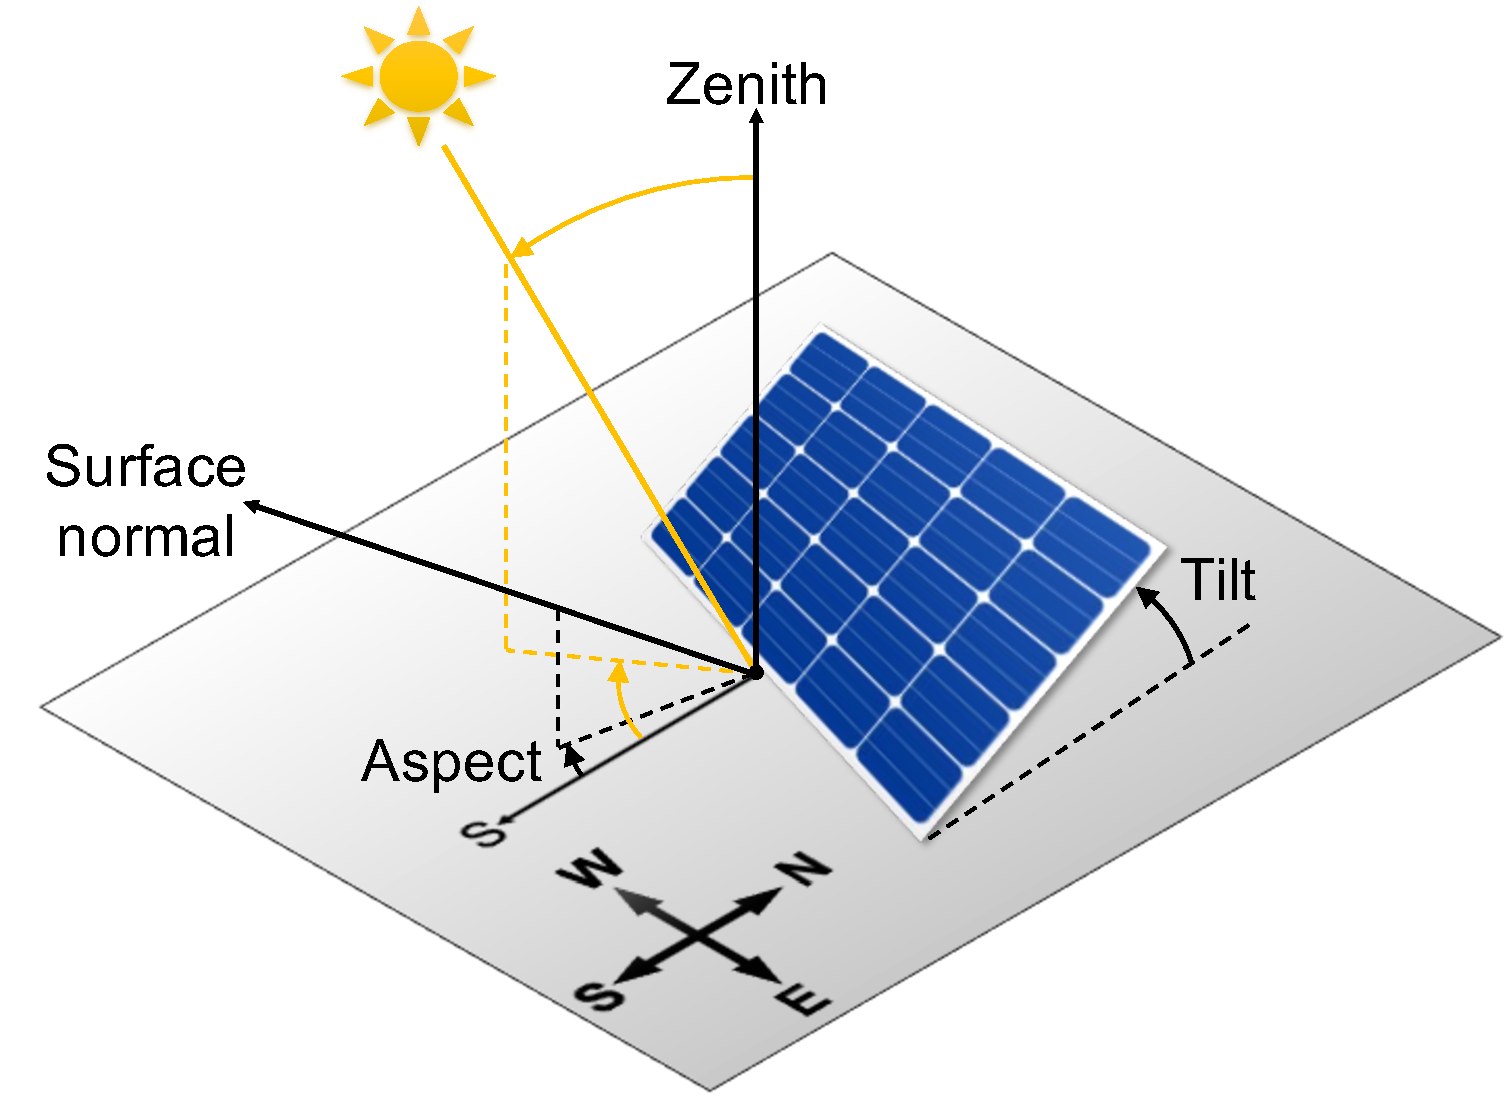
\includegraphics[width=\linewidth]{images/Figs/poa.pdf}  
    \subcaption{}
  \label{figa:solar_geom}
\end{subfigure}
\begin{subfigure}[t]{.53\textwidth}
  \centering
  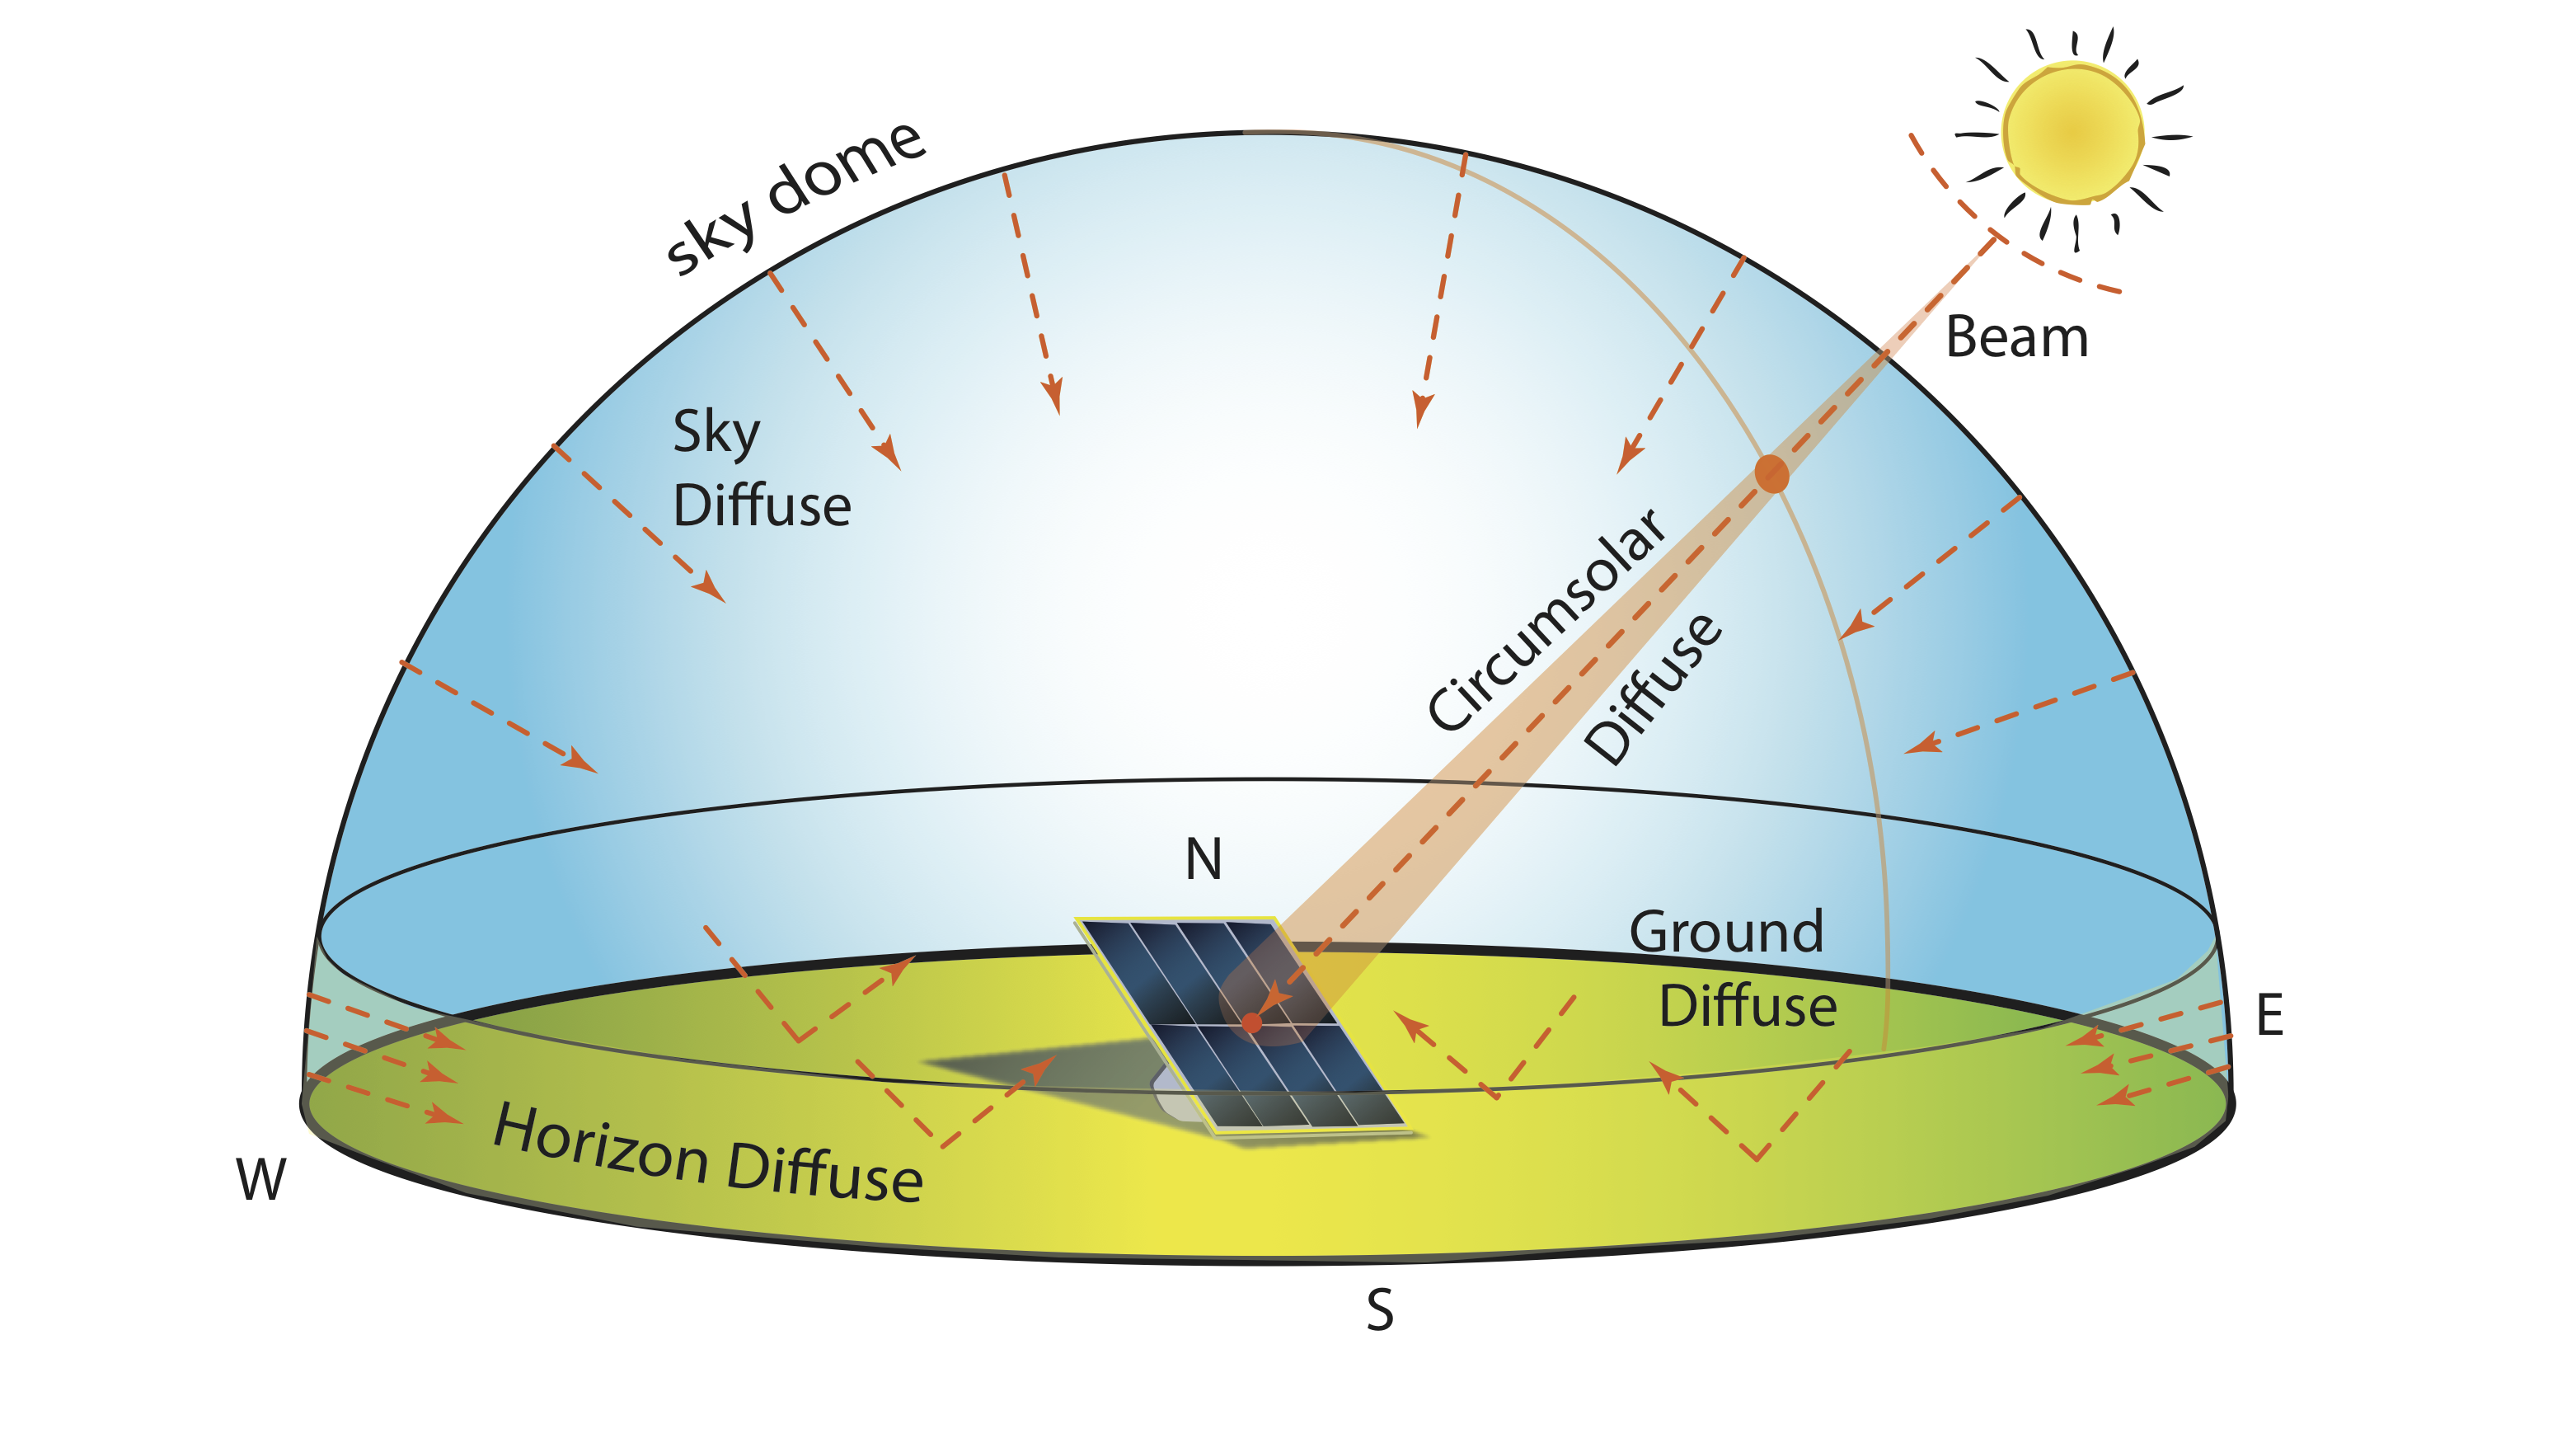
\includegraphics[width=\linewidth]{images/Figs/diffuse_components.png}  
    \subcaption{}
  \label{figb:solar_geom}
\end{subfigure}
\caption{Geometrical models for calculating (a) the angle of incidence of direct beam radiation on a tilted plane, and (b) the isotropic, circumsolar and horizon diffuse components (Source: \citet{brownson_44_nodate}).}
\label{fig:solar_geom}
\end{figure}

To compute the direct, diffuse and reflected tilted irradiance components $G_{Bt}$, $G_{Dt}$ and $G_{Rt}$, empirical and geometrical models are widely accepted in the literature. 
The direct component is obtained from a geometrical projection of the horizontal $G_B$ on the angle of incidence of the sun rays on the tilted panel ($\theta$) (see Fig.~\ref{figa:solar_geom}). Mathematicaly, this projection is defined as \cite{gulin_estimation_2013}:

\begin{equation}
\label{eq:direct}
    G_{Bt} = G_{B} * \max \left( 0, \frac{\cos(\theta)}{\cos(\theta_Z)} \right)
\end{equation}

where
\begin{equation}
\label{eq:dir_angle}
\cos(\theta) = \sin(\beta) \sin(\theta_Z) \cos(\gamma_S - \gamma) + \cos(\beta) \cos(\theta_Z) 
\end{equation}

The angles $\theta_Z$ and $\gamma_S$ describe the sun zenith and azimuth angles, respectively, while roof tilt and aspect are given by $\beta$ and $\gamma$.

Diffuse tilted irradiance is more complex to determine due to its diffracted nature. Several models exist with different assumptions and hence varying complexity. \citet{assouline_estimation_2017} reviews these different models and compares the temporal resolutions for which they are applicable.
Of the methods listed in \citet{assouline_estimation_2017} , the Perez model ~\cite{perez_modeling_1990} is the most frequently used model in the reviewed literature \cite{buffat_scalable_2018,jakubiec_method_2013,mainzer_assessment_2017,wegertseder_combining_2016}, and will also be used throughout this thesis.
The empirical formula for $G_{Dt}$ using the Perez model is given by~\cite{perez_modeling_1990}:

\begin{equation}
\label{eq:diffuse}
G_{Dt} = G_D * \left[ (1 - F_1) \left( \frac{1 + \cos \beta}{2} \right) 
       + F_1 \frac{ a }{ b }
       + F_2 \sin \beta \right]
\end{equation}

where $F_1$ and $F_2$ are empirically fitted functions for the circumsolar and horizon brightness, and $a$, $b$ are geometric angles. The derivation of these factors is described in \cite{loutzenhiser_empirical_2007}. The three addends in Eq.~\ref{eq:diffuse} represent an isotropic component, a circumsolar component originating from the sun disk (modelled as a point source) and a horizon component respectively, as shown in Fig.~\ref{figb:solar_geom}.

The reflected radiation ($G_{Rt}$) is again obtained from a widely used geometric projection based on the surface albedo $\rho$, which is defined as \cite{duffie_solar_2013}:

\begin{equation}
\label{eq:reflected}
G_{Rt} = G_h * \rho \left( \frac{1-\cos \beta}{2} \right)
\end{equation}

To ease the notation, Equations~\ref{eq:direct}-\ref{eq:reflected} can be referred to as:
\begin{equation}
\label{eq:tilted_irrad_simplified}
G_{Bt} = F_B G_B, \quad G_{Dt} = F_D G_D, \quad G_{Rt} = F_R G_h
\end{equation}



\subsubsection{PV module and inverter efficiency}
\label{app:efficiency}

In contrast to the modelling of the POA radiation, a variety of different empirical models exist to compute the electricity yield of PV panels. These methods commonly use the PV cell temperature as input
To model different PV technologies, \citet{buffat_scalable_2018} use 

In this work, the module and inverter efficiencies are computed using the \textit{PVWatts} model developed by the National Renewable Energy Laboratory (NREL) \cite{dobos_pvwatts_2014}. The DC power output of a PV panel is modelled as a function of the tilted radiation $G_t$ and the cell temperature $T_{cell}$:

\begin{equation}
\label{eq:Pdc}
    P_{dc} = \frac{G_{t}}{1000} P_{dc0} (1 + \gamma_{pdc}(T_{cell}-T_{ref}))
\end{equation}

where $P_{dc0}$ is the DC rating of the panel, $\gamma_{pdc}$ is its temperature coefficient and $T_{ref}$ is the reference temperature.
%
We use average panel specifications of mid-range 60-cell mono-crystalline PV modules, the most frequently used technology in Switzerland \cite{buffat_scalable_2018}, from three market-leading manufacturers (JA Solar, Jinko Solar, Trinasolar).
%
The \textit{PVSyst} model~\cite{faiman_assessing_2008} is used to derive $T_{cell}$ from $G_t$ and the ambient temperature $T_{amb}$:

\begin{equation}
    T_{cell} = T_{amb} + G_t \frac{\alpha (1 - \eta_m)}{U}
\end{equation}

where $\alpha$ denoted the absorption coefficient, $\eta_m$ denotes the module efficiency and $U$ is the heat transfer component. 
%
From the DC power output and the area of a PV panel ($A_{panel}$), we compute the module efficiency $\eta_{PV}$:

\begin{equation}
\label{eq:eff}
    \eta_{PV} = \frac{P_{dc}}{G_{t} * A_{panel} }
\end{equation}

The empirical loss formula for the inverter efficiency ($\eta_{inv}$) in \textit{PVWatts} is given by:

\begin{equation}
    \eta_{inv} = \frac{\eta_{nom}}{\eta_{ref}} \left( -0.0162 * \zeta - \frac{0.0059}{\zeta} + 0.9858 \right)
\end{equation}

where $\zeta = P_{dc}/P_{dc0}$, $\eta_{nom}$ is the nominal inverter efficiency and $\eta_{ref}$ is the reference efficiency. 
%
The performance factor ($PF$) is obtained by multiplying $\eta_{inv}$ with other system losses. These include soiling, degradation, mismatch, wiring and connection losses and are estimated as 14\% \cite{dobos_pvwatts_2014}. 

\begin{table}[htbp]
\centering
\footnotesize
\caption{Parameters used in the PV module and inverter efficiency models \cite{dobos_pvwatts_2014, faiman_assessing_2008}.}
\label{tab:efficiency}

    \begin{tabular}{lll}
    \hline
    \textbf{Parameter} & \textbf{Value}     & \textbf{Description}          \\ \hline
    $P_{dc0}$          & $285 Wp$           & Nameplate DC rating           \\
    $\gamma_{pdc}$     & $-0.39\%/ ^\circ C$& Temperature coefficient       \\
    $T_{ref}$          & $25^\circ C$       & Cell reference temperature    \\
    $\alpha$           & 0.9                & Absorption coefficient        \\
    $\eta_m$           & 0.17               & Nominal module efficiency     \\
    $U$                & $15 W/m^2K$        & Heat transfer component       \\
    $A_{panel}$        & $1.6 m^2$          & PV panel area                 \\
    $\eta_{nom}$       & 0.96               & Nominal inverter efficiency   \\
    $\eta_{ref}$       & 0.9637             & Reference inverter efficiency \\ \hline
    \end{tabular}
\end{table}

We use the \texttt{pvlib} python package developed by Sandia National Laboratories \cite{holmgren_pvlib_2018} for the computing the POA irradiance and the module and inverter efficiency. All parameter values are shown in Table~\ref{tab:efficiency}.

\subsection{Geospatial techniques}
\label{GIS_methods}

\subsubsection{Shading effects and sky view factor}

\begin{figure}[htb]
	\centering
	\begin{subfigure}[t]{.49\textwidth}
		\centering
		% include second image
		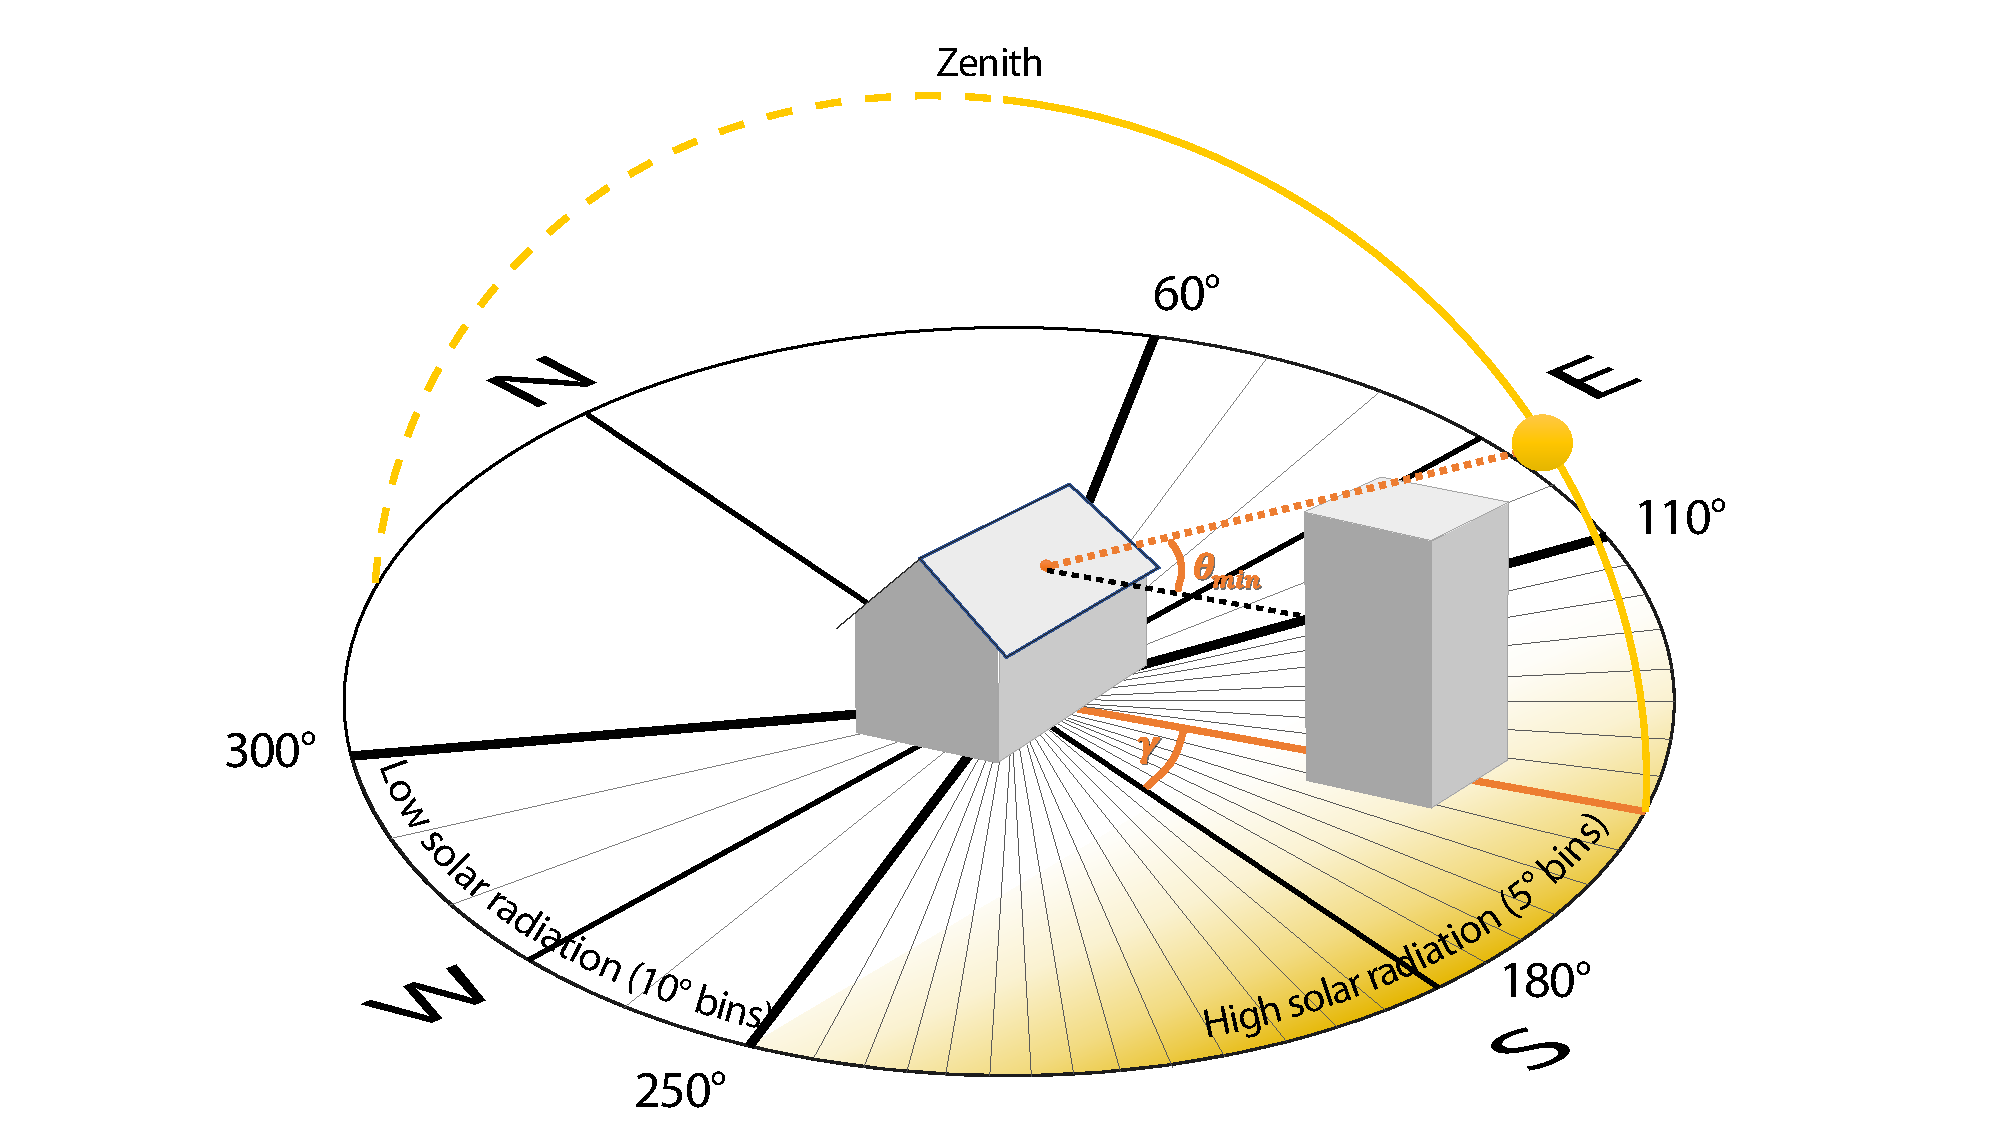
\includegraphics[trim=100 0 130 0, clip, width=.9\linewidth]{Figs/horizon.pdf}  
		\subcaption{}
	\end{subfigure}
	\begin{subfigure}[t]{.49\textwidth}
		\centering
		% include second image
		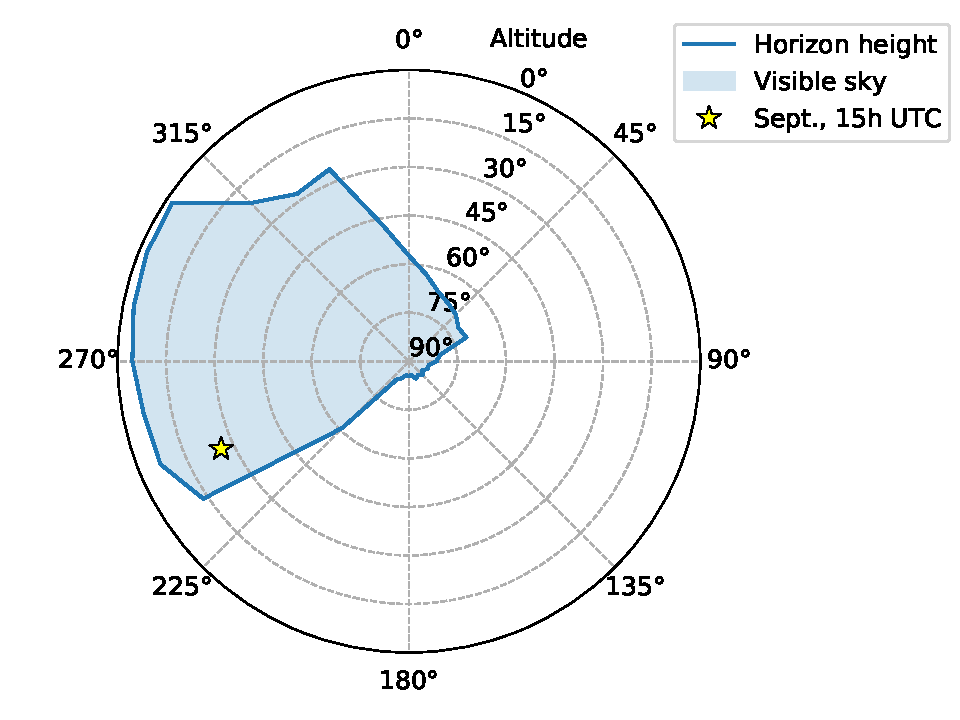
\includegraphics[width=\linewidth]{images/Figs/skyview_point_w_star.pdf}  
		\subcaption{}
		\label{figb:horizon_method}
	\end{subfigure}
	\caption{Viewshed horizons for an example roof, (a) conceptual graph with relevant horizon bins for quantification of shading effects, (b) polar plot of horizon height and visible sky proportion ($\mathit{SVF} = 0.3$), with an example sun position for Switzerland (September, 15h UTC).}
	\label{fig:horizon_method}
\end{figure}

\begin{figure}[htb]
	\centering
	\begin{subfigure}{.49\textwidth}
		\centering
		% include second image
		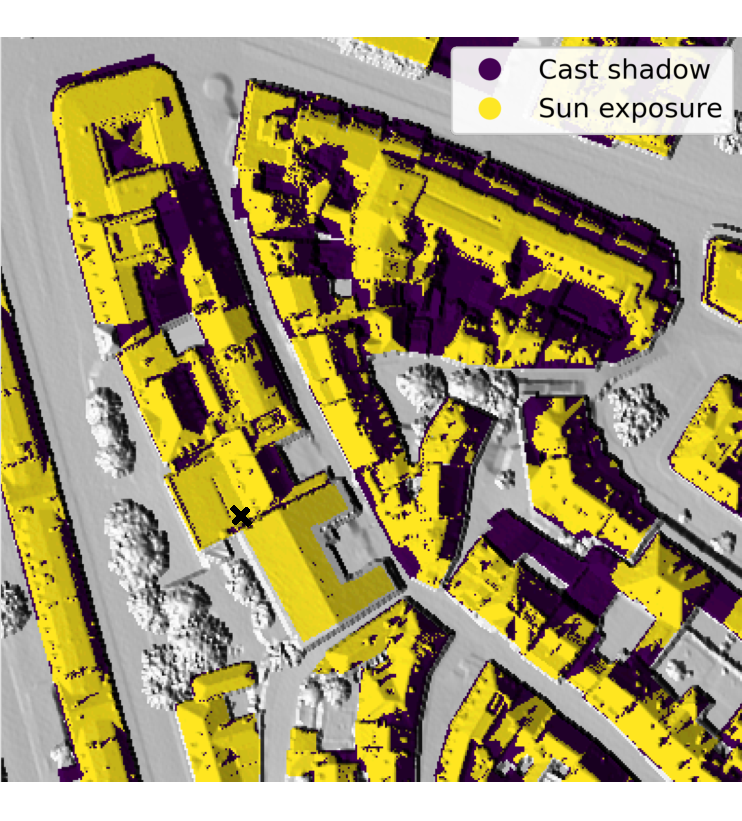
\includegraphics[height=.9\linewidth]{images/Figs/demo_vis_09_15h_w_cross.pdf}  
		\subcaption{}
	\end{subfigure}
	\begin{subfigure}{.49\textwidth}
		\centering
		% include second image
		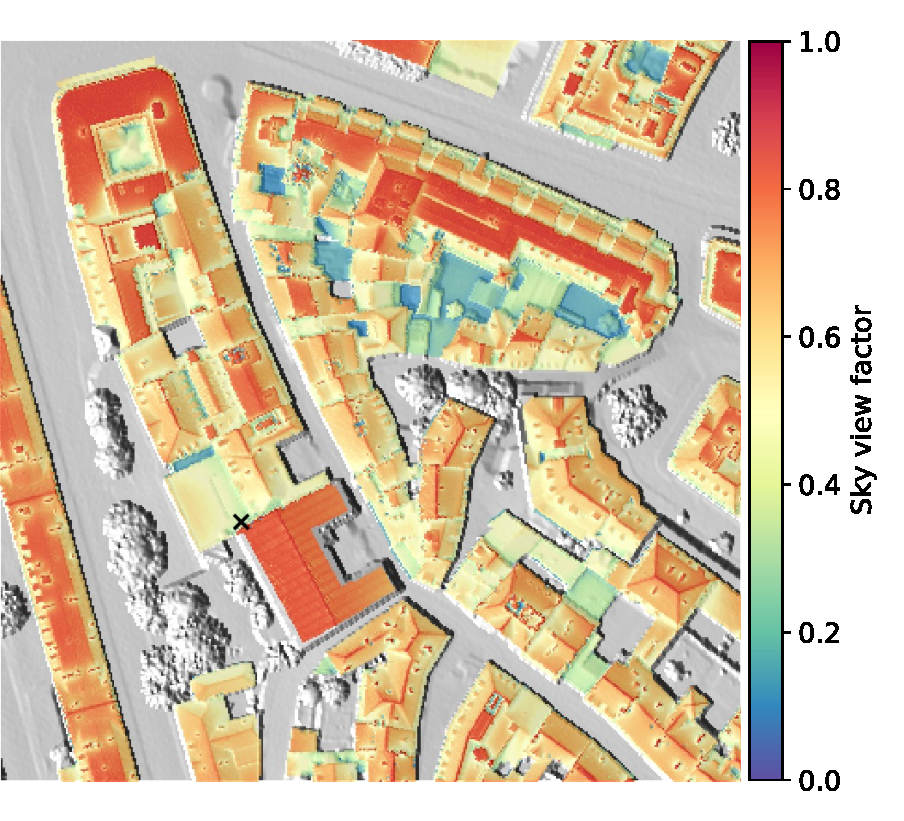
\includegraphics[height=.9\linewidth]{images/Figs/svf_w_legend.pdf}  
		\subcaption{}
	\end{subfigure}
	\caption{Raster-based (a) cast shadows for one example hour (15h UTC in September, see star in Fig.\ref{figb:horizon_method}) and (b) sky view factor for an area of $200\times200$ m$^2$ in Geneva, Switzerland. The cross on the figures shows the point for which the horizon map is shown in Fig.\ref{figb:horizon_method}.}
	\label{fig:raster_svf_ssh}
\end{figure}


To quantify the shading effects, we use GIS to compute horizon maps from a Digital Elevation Model (DEM). 
The horizon describes the minimum sun elevation angle required to illuminate each pixel of the DEM. 
Horizon maps are computed for each azimuth angle of the sun (see Figure~\ref{fig:horizon_method} for one example point). From the horizon maps, a binary shading mask of the surface can be derived for each time step, where a $0$ represents a shaded cell, and a $1$ represents a cell that is exposed to the sun.

The derivation of $C_{sh}$ requires a threshold which defines the suitability of a surface for PV installation. Possible fractions of unsuitable area due to shading are compared in~\cite{wiginton_quantifying_2010}. As the reported values vary largely, we redefine the threshold based on our data. We rate all areas that exhibit a lower-than-average direct sun exposure unsuitable for PV. These areas define the \textit{shaded area coefficient}. The threshold is found by averaging the binary shading masks of 150 non-zero time steps (where the sun is above the horizon), as shown in Figure~\ref{fig:horizons}c. Across all time steps and all roof surfaces, the average sun exposure is 42.7\%, so we choose a rounded threshold of 40\%.

The $S_{sh}(t)$ is computed for each time step $t$ as the ratio of the number of illuminated pixels (pixel value $1$ in the binary shading mask) over the total number of pixels with an average sunlight exposure $> 40\%$. The full GIS algorithm is summarized in Algorithm~\ref{alg:shade}. 

The sky view factor (SVF) represents the visible proportion of the sky and is computed from the same horizon maps as the shading effects.

\begin{comment}
\subsection{Solar thermal heat generation}

The computation of the technical potential of a solar thermal collector is more complex to compute, as the solar thermal collector is typically coupled with a heat pump and a hot water tank. In the thermal application, the temperature of the collector and the ambience also play a larger role. Some studies still consider a constant efficiency value [27], while several studies suggest to consider temperature and incident irradiance [11], [28], [29].
\end{comment}

\subsubsection{Available area for solar panel installation}


Based on the an early study of RPV potential in Europe \cite{iea_potential_2002}, we identify three factors of the rooftop available area that are accounted for in different ways in the literature, namely (i) the total roof area, (ii) the roof exposure or suitability and (iii) the roof utilisation. 

\begin{comment}
% For individual roofs, panels can be custom-fitted based on aerial photographs ~\cite{ordonez_analysis_2010} to realistically estimate the maximum available area, taking into account the rooftop geometry as well as any obstructing objects inhibiting the placement of solar panels (roof superstructures).
% Custom-fitting however is not scalable to entire cities or regions, requiring either image processing \cite{mainzer_assessment_2017} or high-resolution 3D building models \cite{engel_effiziente_nodate} for a detailed estimation of the available area.
% As the required input data is not available for many study areas and the computational time for these methods may be prohibitively high, approximative approaches are widely used in the literature.
These range from using standard tabulated factors based on expert opinions [26], statistical methods [7] and extrapolation techniques based on Machine Learning [3]. Assouline et al. [14] provide a detailed analysis of these methods. 

Focus primarily on radiation: Buffat, Desthieux; compute for individual systems: Calcabrini; 
Wegertseder: 25\% of useful roof area for res., 30\% for housing blocks, 50\% for high-rise towers

strzalka: manually excluding roofs with windows etc., otherwise using all areas

exclude small areas and strongly shaded areas: Hong (per time step)

Thus, many studies employ constant value methods \cite{assouline_estimation_2017}, which assume a constant ratio of available area. 
These ratios may be formulated with reference to territorial areas or population count \cite{izquierdo_method_2008,iea_potential_2002,wiginton_quantifying_2010,bodis_high-resolution_2019}, based on building prototypes \cite{wegertseder_combining_2016} or formulated as a constant fraction of individual roofs~\cite{portmann_sonnendach.ch:_2016}. 
In studies where detailed roof data is available through building cadastres 
Full rooftops \cite{bodis_high-resolution_2019}, rooftop avail area fraction ()

The geospatial algorithm is used to virtually install PV panels on the tilted roofs by projecting rectangular polygons onto these surfaces, as shown in Fig.~\ref{fig:panels}c. 
The starting point for this process are the roof polygons and superstructures (Fig.~\ref{fig:panels}a). Panels are installed on the grey areas in Fig~\ref{fig:panels}b, after superstructures (if applicable) and a buffer of 40cm are removed from the polygons~\cite{assouline_large-scale_2018}. The panels are installed in adjacent rows along the roof aspect, starting from the bottom left corner, as described in Algorithm \ref{alg:panels}. It is implemented using the python \texttt{geopandas} library \cite{kelsey_jordahl_geopandas/geopandas:_2019}.

Virtual PV panels were placed in both horizontal and vertical alignments, as no alignment has technical advantages over the other and both are widespread. The alignment that allows the higher number of panels to be installed on each roof is selected as final panel alignment. 
\end{comment}

\section{Shallow geothermal energy}
\label{geo_method}

This section provides an overview of the concept behind the estimation of the technical potential for borehole heat exchangers (BHE). It introduces the parameters used in the estimation (Section \ref{geo_params}) and summarizes the analytical methods for simulating the thermodynamic processes in the ground, which form the basis for the potential estimation (Section X, XX). Different analys

In this work, the technical geothermal potential for BHSs is defined as:

\textbf{The heat energy ($E_Q$) that may be \textit{sustainably} extracted from a field of BHEs, each of length $H$ and spaced apart by a distance $B$, by a ground source heat pump (GSHP) system with a heat extraction power $Q$ during an annual operational time $t_{op}$. }

The key condition for a \textit{sustainable} extraction of energy from the ground is to keep the mean temperature of the borehole fluid above the freezing temperature ($-1.5^\circ C$ \citep{wagner_erdsondenpotenzial_2014}) during the time of operation. This condition is a limiting factor on the total heat that can be extracted from the ground and plays a key role in the estimation of the large-scale BHE potential estimation.

With appropriately dimensioned and spaced boreholes, a large-scale potential can be defined in $kWh/m^2$. This potential may be computed at annual temporal scales (using an annual mean heat extraction rate), at monthly scales (using the heat degree days as weighting function) or at hourly scales (using hourly load profiles).
The aim here is to define a maximum amount of energy that can be extracted from the ground without negatively affecting the long-term ground temperature. Energy demand is on purpose not taken into account. 
This is due to the fact that multiple operation modes exist, e.g. individual BHEs or entire fields that are connected to heat distribution networks. The separation between supply and demand also allows to simulate scenarios of "hybrid" systems, where the demand is covered by different sources.

\begin{figure}
    \centering
    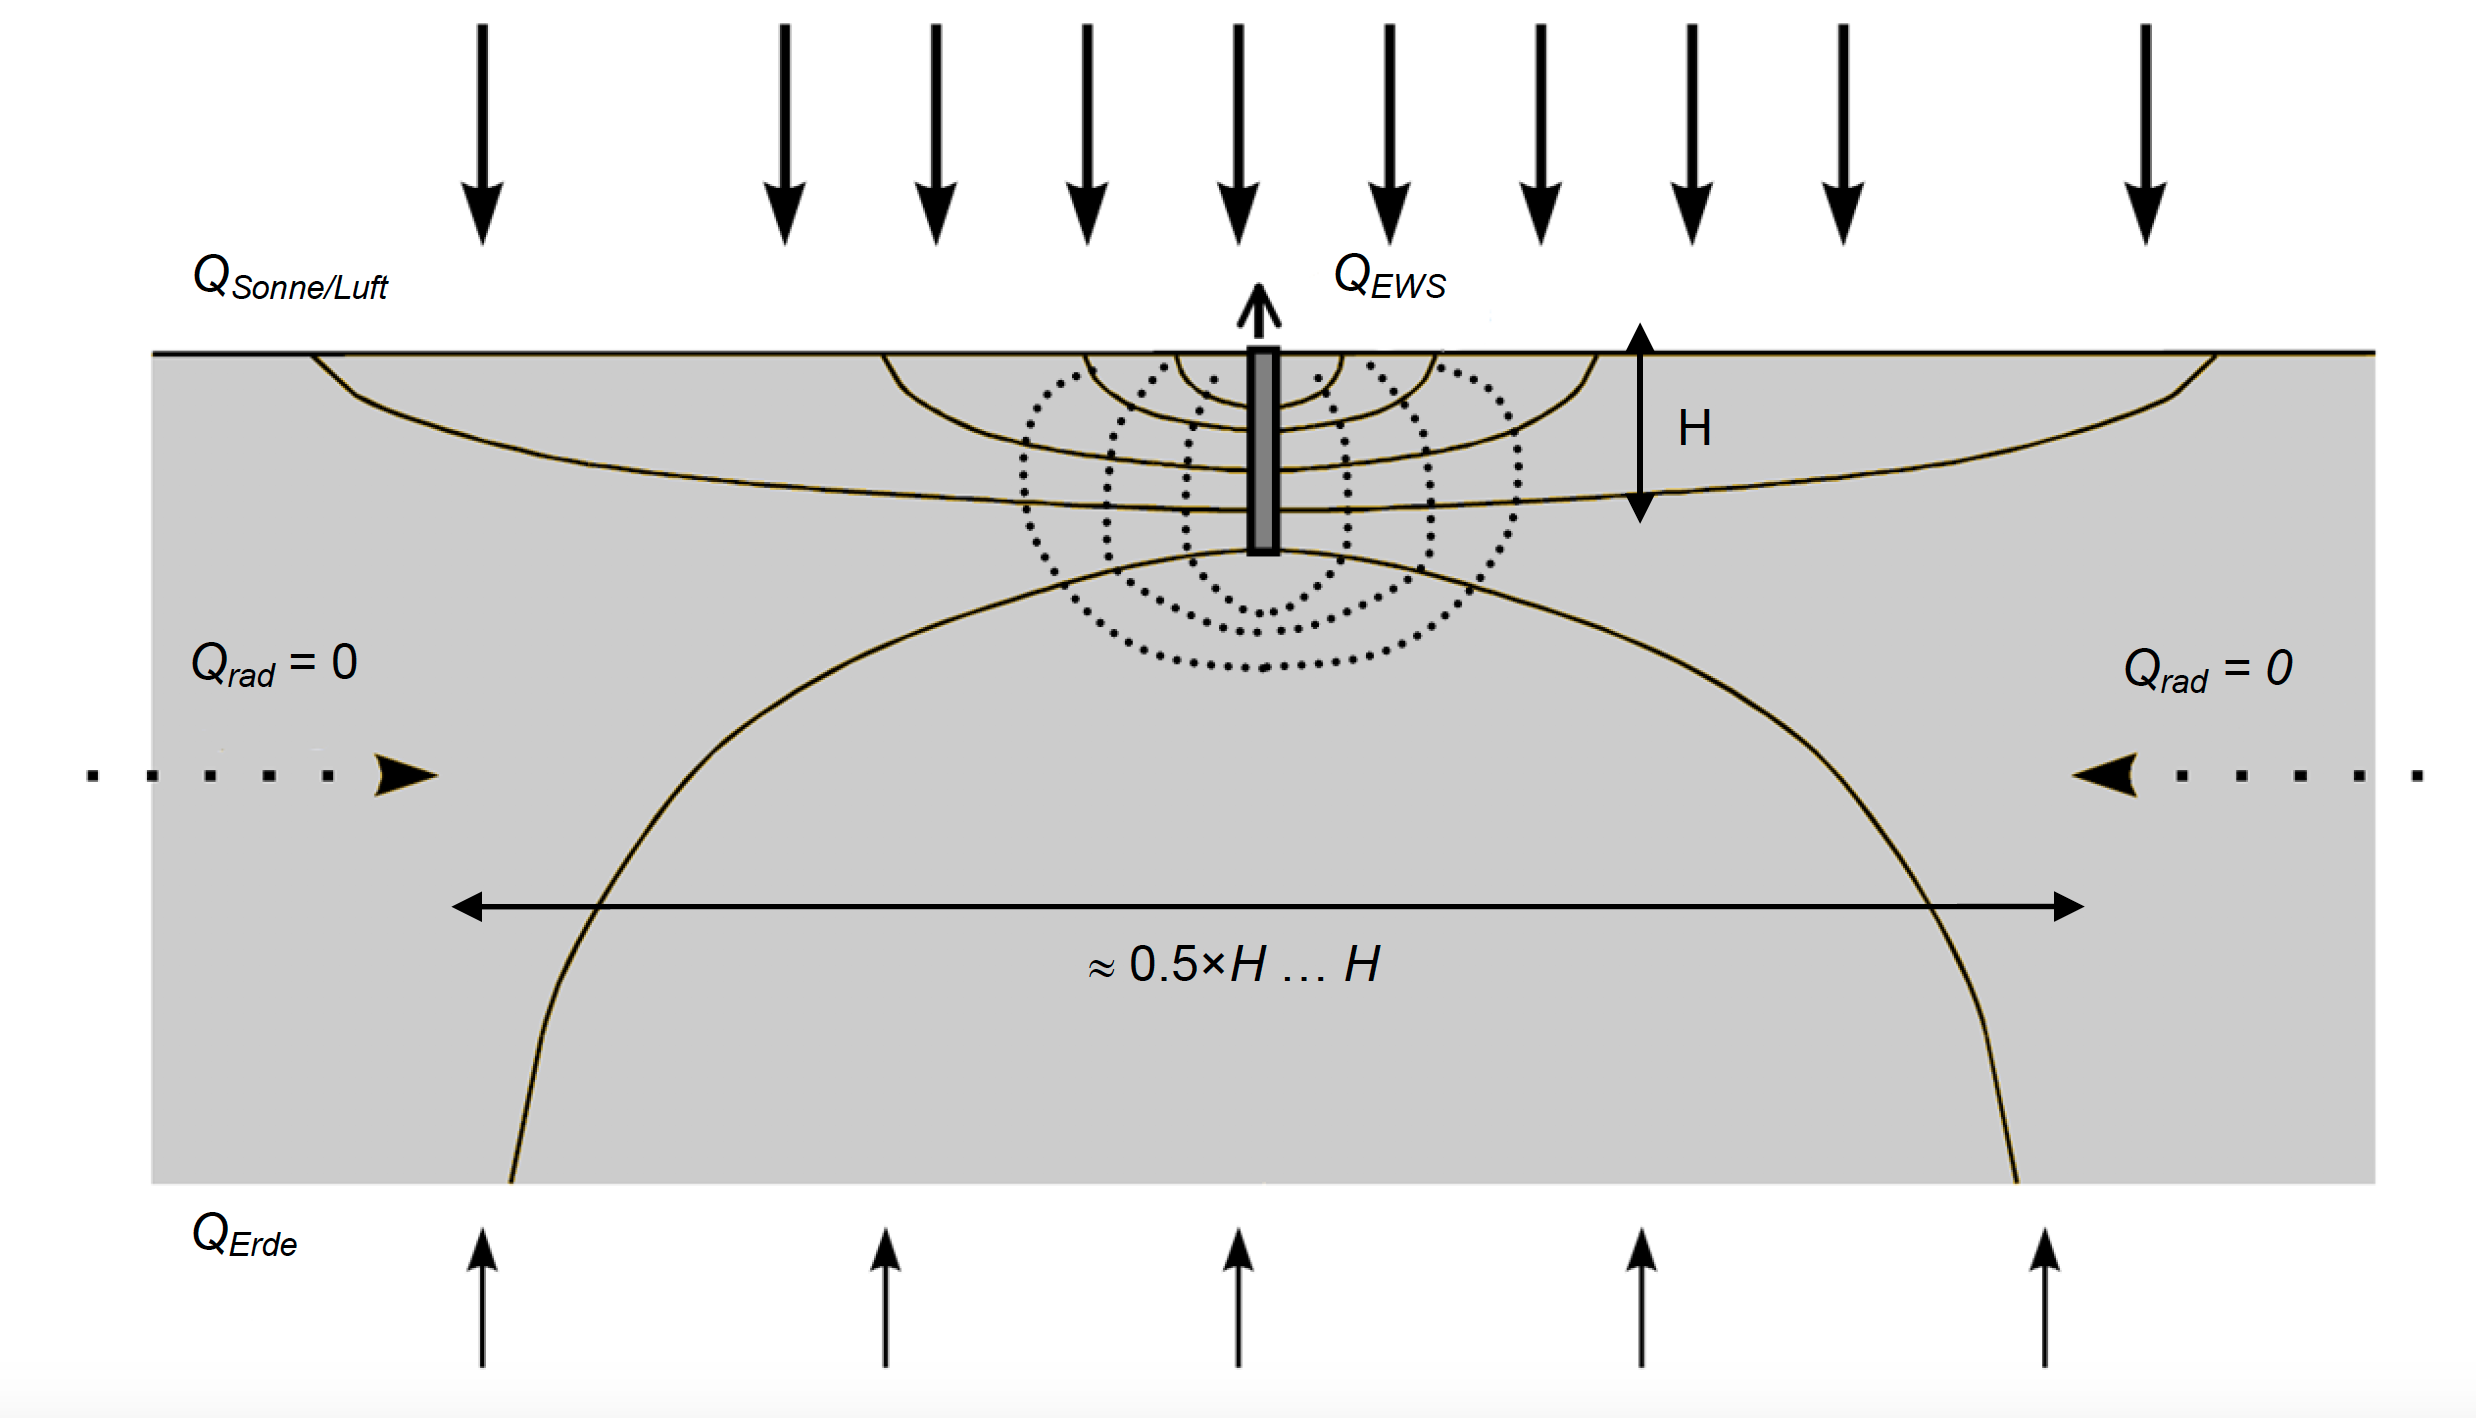
\includegraphics[width=0.7\linewidth]{Figs/BHE_layout.png}
    \caption[Single BHE installation and its effects on the temperature in the ground.]{Single BHE installation and its effects on the temperature in the ground. The arrows on the top indicate the natural heat flux from the environment, those on the bottom indicate the geothermal heat flux. The dashed lines are isothermal lines, while the continuous lines represent the heat flow in the stationary state. Source: \citet{wagner_erdsondenpotenzial_2014}}
    \label{fig:BHE}
\end{figure}

This report summarizes the methods used to quantify the impact of a BHE installation on the short-term and long-term temperature in the ground, and consequently on the temperature of the heat extraction fluid inside the borehole. The case of a single borehole is shown in Fig.~\ref{fig:BHE}. The heat extracted by the borehole of length $H$ (in the center) leads to a temperature drop in the ground. This effect reduces with the distance $r$ to the center of the borehole, as indicated by the dashed lines that represent isothermal conditions. The temperature drop does not happen instantly, but the temperature reduces gradually over the years, until a \textit{steady state} is reached. In the steady state, the extracted heat equals exactly the energy flux from the environment (the air and sun on the surface, and the geothermal heat flux in the ground). The heat flow in this stationary state is shown by the continuous lines in Fig.~\ref{fig:BHE}. As a rule of thumb, the radius around the borehole which is impacted by the temperature drop in steady state is between $H/2$ and $H$. At distances further away from the borehole, the temperature drop can always be neglected \cite{pahud_geothermal_2002}, p. 49.

For typical BHE's of 100-250m, it takes a hundred years or more to reach this stationary state (see formula below). However, typical BHE installations are designed to be decommissioned after 50 years \citep{sia_sondes_2010}. In general, it is hence sufficient to fulfill the temperature requirement (see \ref{definition}) for the first 50 years of operation. This means that in practice it is still possible to install boreholes at distances of less than $H/2$, but numerical models are necessary to accurately quantify a distance which sustains a sufficient ground temperature in the planning horizon of 50 years.

The general intuition for the relationship between the spacing of boreholes, the length of the boreholes, the ground temperature and the heat extraction power is the following:
The closer boreholes are placed to each other, the stronger are they impacting each other, which results in a lower ground temperature. 
This lower ground temperature may cause the temperature of the heat carrier fluid to drop below the minimum allowed value; to prevent that, the heat extraction power must be reduced. 
In order to sustain a given heat extraction power and keep a close spacing between boreholes, the depth of the boreholes can be increased. This increases the ground volume from which heat is extracted, but may not be possible due to the ground materials or regulations. 
On the other side, a shorter borehole length means that heat is extracted at a higher rate, which also increases the temperature drop. This can be compensated by either reducing the heat extraction power (which lowers the efficiency of the system) or by increasing the borehole spacing.

\subsection{Parameters}
\label{geo_params}
The parameters involved in the modelling of the thermodynamic behaviour of borehole heat exchangers can be divided into three groups: 

\begin{enumerate}
\item \textbf{Physical parameters} are determined by the geological and hydrological conditions of the ground, and subject to various large-scale studies. Seasonal effects are neglected, as boreholes typically have a length $> 50m$, which is far beyond the penetration depth of seasonal variations in the ground.

\item \textbf{Technical parameters} are derived from the materials and the technology of the BHEs. We use norm values found in the literature as constants and do not address the impact of variations in the technical parameters on the BHE potential.

\item \textbf{Design parameters} are related to the dimensioning of the boreholes and the borehole fields, in order to estimate a \textit{sustainable} BHE potential. These parameters and the impact of their variation on the BHE potential are the main subject of the analysis. 
\end{enumerate}

We refer to $z$ (in $m$) for the depth in the ground, $r$ (in $m$) for the radial distance to the center of a BHE, $t$ (in $h$ or $a$) for the time and $T$ (in $^\circ C$ or $K$) for the temperature. 

\begin{table}[b]
\footnotesize
\caption{Physical parameters. Norm values and ranges for Switzerland are obtained from \citep{sia_sondes_2010}.}
\label{tab:phys_params}

\centering
\begin{tabular}{lllll}
\hline
\textbf{Symbol}             & \textbf{Unit} & \textbf{Description}           & \textbf{Formula}                                      & \textbf{Norm value / range (CH)} \\ \hline
$\lambda$                   & $W/mK$        & Thermal conductivity           &                                                       & $1-4$ (Plateau: $2-3$)           \\
$\alpha$                    & $m^2/s$       & Thermal diffusivity            & $\alpha = \frac{\lambda}{\rho C}$                     & $0.9-1.4 \times 10^{-6}$         \\
$\rho C$                    & $MJ/m^3K$      & Volumetric heat capacity       &                                                       & $1.2-3.5$ (Plateau: $2-2.5$)     \\ \hline
$T_g(z)$                    & $^\circ C$    & Undisturbed ground temperature &                                                       & \textit{Norm}: 10                         \\
$\frac{\Delta T}{\Delta z}$ & $K/m$         & Temperature gradient           & $T_g(z) = T_0 + z * \frac{\Delta T}{\Delta z} $       & Plateau: 0.03, Alps: 0.025       \\
$T_0$                       & $^\circ C$    & Surface temperature            &                                                       & \textit{Norm}: 8.5                        \\ \hline
$\dot{q}_{g}$               & $mW/m^2$      & Geothermal heat flow           & $\dot{q}_{g} = \lambda * \frac{\Delta T}{\Delta z}$   & $40-170$                         \\ \hline
\end{tabular}
\end{table}

\textbf{Physical parameters}. The physical parameters are listed in Table~\ref{tab:phys_params}. The \textit{thermal conductivity} $\lambda$ and \textit{thermal diffusivity} $\alpha$ are used in the numerical models. However, the geological properties of different types of rocks are typically provided as $\lambda$ and the \textit{volumetric heat capacity} $\rho C$. For a reference table, see \cite{pahud_geothermal_2002}, p.30 or \cite{sia_sondes_2010}, p.39. From these parameters, the thermal diffusivity is computed as:

\begin{equation}
    \alpha = \frac{\lambda}{\rho C}
\end{equation}

Another important physical parameter is the \textit{undisturbed ground temperature} $T_g(z)$. In particular, the temperature at half of the borehole depth ($z = H/2$) is of interest. If no data is available for estimating $T_g$ directly, it can be extrapolated from the \textit{surface temperature} $T_0$ and the \textit{temperature gradient} $\Delta T/\Delta z$: 

\begin{equation}
    T_g(z) = T_0 + z * \frac{\Delta T}{\Delta z}
\end{equation}

\begin{figure}
    \centering
    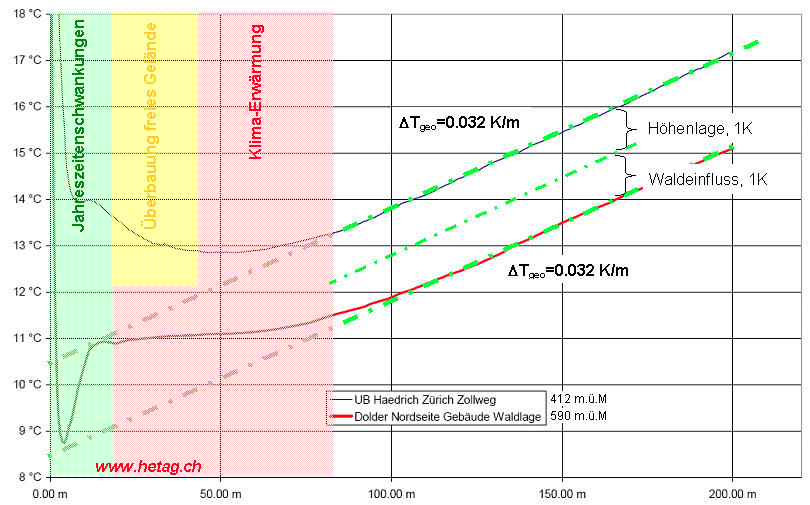
\includegraphics[width=0.6\linewidth]{Figs/ground_temperature.png}
    \caption[Example for the variation in ground temperature for two measurements of ground temperature in Zürich.]{Example for the variation in ground temperature for two measurements of ground temperature in Zürich, showing the influence of altitude and additional surface heating. Source: \citet{huber_bodentemperaturen_2014}.}
    \label{fig:T_ground}
\end{figure}

An analysis of different methods to determine $T_0$ is performed in \citep{signorelli_geoscientific_2004} (Chapter 5). In general, the mean annual surface temperature can be approximated from the mean annual ambient temperature $\overline{T_{amb}}$ by adding a difference term ($\Delta T_0$) that depends on the altitude ($z_0$). As the actual ground temperature may vary, the SIA norm instructs the addition of a tolerance ($\Delta T_{H/C}$), such that \citep{sia_sondes_2010}: 

\begin{equation}
    T_0 = \overline{T_{amb}} + \Delta T_0 + \Delta T_{H/C} 
\end{equation}

\begin{equation*}
    \Delta T_0 = \left\{
        \begin{matrix}
            1.55 & z_0 < 1000m \\ 1.55 + \frac{z_0 - 1000}{800} * 2.45 & z_0 > 1000m
        \end{matrix} \right. , \quad 
    \Delta T_{H/C}  = \left\{
        \begin{matrix}
            - 1 K & heating\ (H) \\ +1 K & cooling\ (C)
        \end{matrix} \right.    
\end{equation*}

Two examples for an unconsidered variation are shown in Fig.~\ref{fig:T_ground}. The presence of forests (red line) results in the ground temperature being approximately $1K$ lower than that expected from $\overline{T_{amb}}$. \citet{huber_bodentemperaturen_2014} states that, on the other hand, areas with high snow coverage may be up to $4K$ warmer than expected. The second example (black line) shows a case where the actual ground temperature is $1K$ higher than expected due to an altitude difference between the BHE and the weather station. In the Swiss plateau, this difference is approximately $0.47 K$ per $100m$ altitude increase with respect to the weather station \citep{huber_bodentemperaturen_2014}.
As the ground temperature in fact reflects the ambient temperature of the past, historic measurements should be used to determine the annual mean ambient temperature \citep{huber_bodentemperaturen_2014}. 

A final parameter to keep in mind is the (undisturbed) \textit{geothermal heat flow} $\dot{q}_{g}$. It is given by:

\begin{equation}
    \dot{q}_{g} = \lambda * \frac{\Delta T}{\Delta z}
\end{equation}

The geothermal heat flow is approximately constant across the outer crust of the earth, but may vary in mountain terrain \citep{huber_bodentemperaturen_2014}. This means that a high thermal conductivity  implies a low temperature gradient, and vice versa. The relationship may hence be used to compute $\lambda$ or $ \frac{\Delta T}{\Delta z}$ if other data is unavailable. A map of geothermal heat flows in Switzerland is shown in Fig.~\ref{fig:q_geo}. It was created by Medici and Rybach in 1995 and updated by Sachs and Eberhard in 2010\footnote{The data is now available as open data at:\\ \url{https://opendata.swiss/de/dataset/geothermische-karte-der-schweiz-1-500000}}.

\begin{figure}
    \centering
    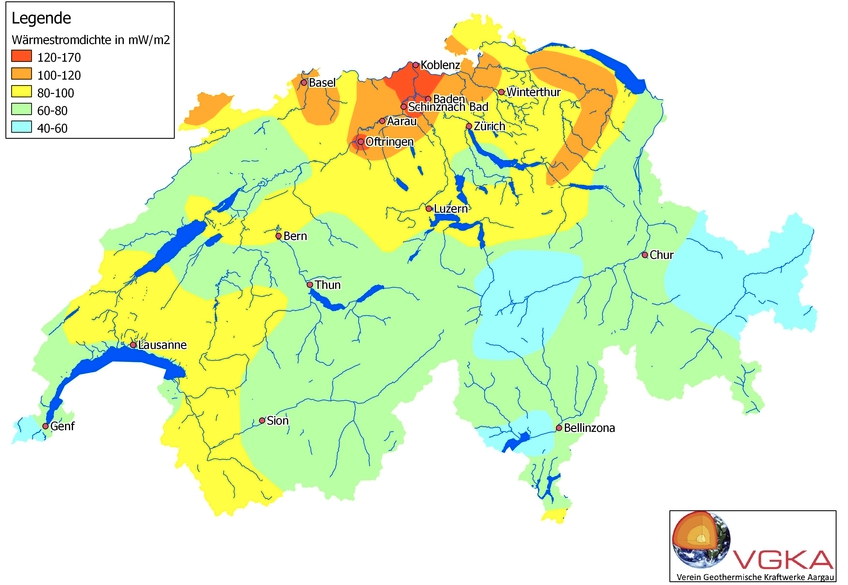
\includegraphics[width=0.6\linewidth]{Figs/q_geo.png}
    \caption[Map of geothermal heat flows in Switzerland]{Map of geothermal heat flows in Switzerland \citep{huber_bodentemperaturen_2014}.}
    \label{fig:q_geo}
\end{figure}

\begin{figure}[b]
    \centering
    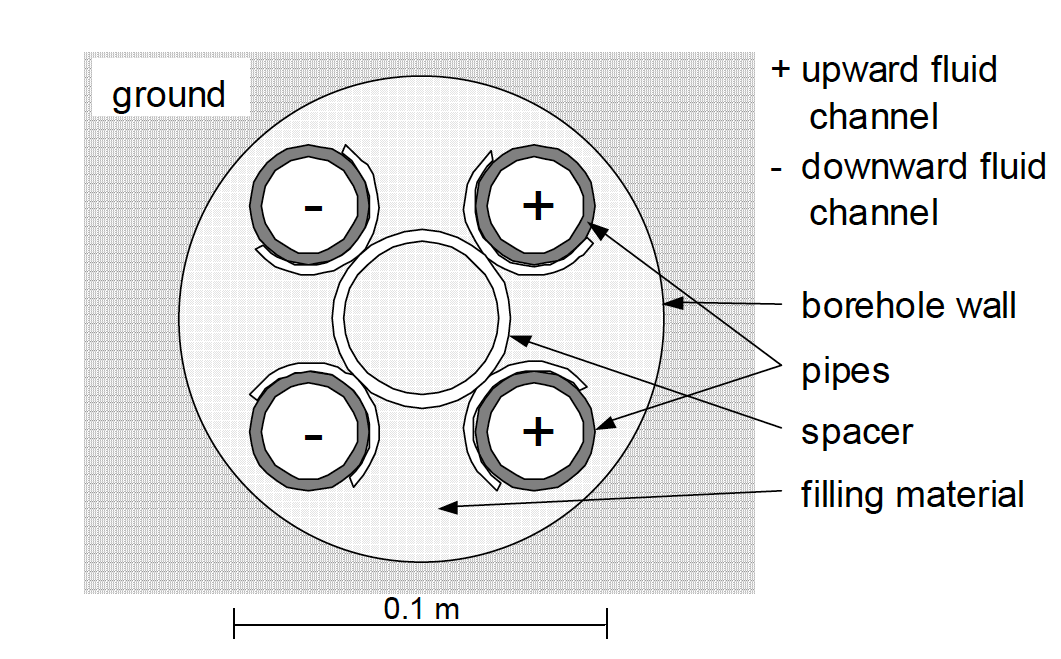
\includegraphics[width=0.4\linewidth]{Figs/BHE_tech.png}
    \caption[Cross-section of a duplex BHE layout.]{Cross-section of a duplex BHE layout \citep{wagner_erdsondenpotenzial_2014}.}
    \label{fig:BHE_cross-sec}
\end{figure}

\textbf{Technical parameters}. The technical parameters required to determine the large-scale geothermal potential as defined in \ref{definition} are taken as constants based on examples in the literature. The mean fluid temperature inside the borehole ($T_{f, min}$) is set according to \citet{sia_sondes_2010} at $-1.5^\circ C$. To fulfill this condition, the temperature drop inside the borehole needs to be estimated. This requires knowledge of the borehole radius ($r_B$) as well as the effective thermal resistance of the borehole ($R_b^*$). A typical layout of a duplex system, the most common form of BHE installations (\cite{sia_sondes_2010}), is shown in Fig.~\ref{fig:BHE_cross-sec}. The thermal resistance is determined by the materials and the geometry of the BHE, which are analysed in detail in \citep{huber_erdwarmesonden_2005} (Section 4). We use standard values from examples of the literature as summarized in Table~\ref{tab:tech_design_params}.

\textbf{Design parameters}. Two groups of design parameters are relevant to study the multi-fold effects between the geometry of a BHE field and the temperature in the ground, which is typically assessed after a planning horizon $t_{dim}$. 
The first group of parameters are related to the borehole geometry. These include the borehole length/depth ($H$), the horizontal distance between BHEs ($B$) and the distance between the top part of the BHE (where heat is extracted) and the ground surface ($D$). 

A second group of design parameters is related to the heat extraction from the borehole. It includes the heat extraction power ($Q_{HP}$), the maximum heat extraction rate ($q_{max}$), the operating time ($t_{op}$) and the duration of maximum operation ($t_{peak}$). The heat extraction power is related to the power rating of the heat pump (HP), whose typical values are shown in Table~\ref{tab:tech_design_params}. In a large-scale study, however, $Q_{HP}$ is not a technical parameter, as the number of heat pumps in the system is undefined. The heat extraction rate is computed from $Q_{HP}$ and $H$ as given in Table~\ref{tab:tech_design_params}. Nominal curves for $q_{max}$ as a function of $\lambda$ and $\rho C$ are shown in Fig.~\ref{fig:t_q_norm}a. If these are used, $Q_{HP}$ needs to be computed by rearranging the equation for $q_{max}$. The operating time indicates the number of hours in which the heat pump is operating (with power $Q_{HP}$). It changes with altitude and location, and the nominal values are shown in Fig.~\ref{fig:t_q_norm}b. The duration of the peak extraction pulse ($t_{peak}$) measures the maximum time of non-stop operation of the HP, which impacts the maximum temperature drop in the BHE and is usually taken as 1, 5 or 10 days.

\begin{table}[t]
\footnotesize
\caption{Technical and design parameters. Norm values are given in \citep{sia_sondes_2010}, while other parameters are obatined from related studies \citep{pahud_geothermal_2002, wagner_erdwarmesonden._2019, claesson_conductive_1988}.}
\centering
\begin{tabular}{lllll}
\hline
\textbf{Symbol} & \textbf{Unit} & \textbf{Description}                   & \textbf{Formula}                                        & \textbf{Norm value / range (CH)} \\ \hline
$T_{f, min}$    & $^\circ C$    & Minimum mean fluid temperature         & $T_{f} = \frac{T_{in} + T_{out}}{2}$                    & \textit{Norm}: $- 1.5$           \\
$r_b$           & $m$           & Borehole radius                        &                                                         & $0.055-0.07$                      \\
$R_b^*$         & $mK/W$        & Effective borehole resistance          &                                                         & $0.08-0.1$                       \\ \hline
$H$             & $m$           & Borehole depth                         &                                                         & \textit{Norm}: $100$ (typically $100-200$)          \\
$D$             & $m$           & Distance between $z=0$ and BHE outlet  &                                                         & $2-5$                              \\
$B$             & $m$           & Spacing between BHEs                   &                                                         & $>5$ (no effect for $B > H$)     \\ \hline
$Q_{HP}$        & $W$           & Heat extraction power during operation &                                                         & $4500-8400$                      \\
$q_{max}$       & $W/m$         & Maximum heat extraction rate           & $q_{max} = \frac{Q_{HP}}{H}$                            & \textit{Norm}: $20-55$ (Fig.~\ref{fig:t_q_norm}a)           \\
$t_{op}$        & $h$           & Annual operation time                  &                                                         & \textit{Norm}: $1850$ (Fig.~\ref{fig:t_q_norm}b)  \\
$t_{peak}$      & $h$           & Duration of maximum extraction pulse   &                                                         & $1 - 10$ days                    \\ 
\hline
$t_{dim}$       & $a$           & Planning horizon for dimensioning the BHE   &                                                         & $50$                    \\ 
\hline
\end{tabular}
\label{tab:tech_design_params}
\end{table}

\begin{figure}[b]
\centering
\begin{subfigure}{.48\textwidth}
  \centering
  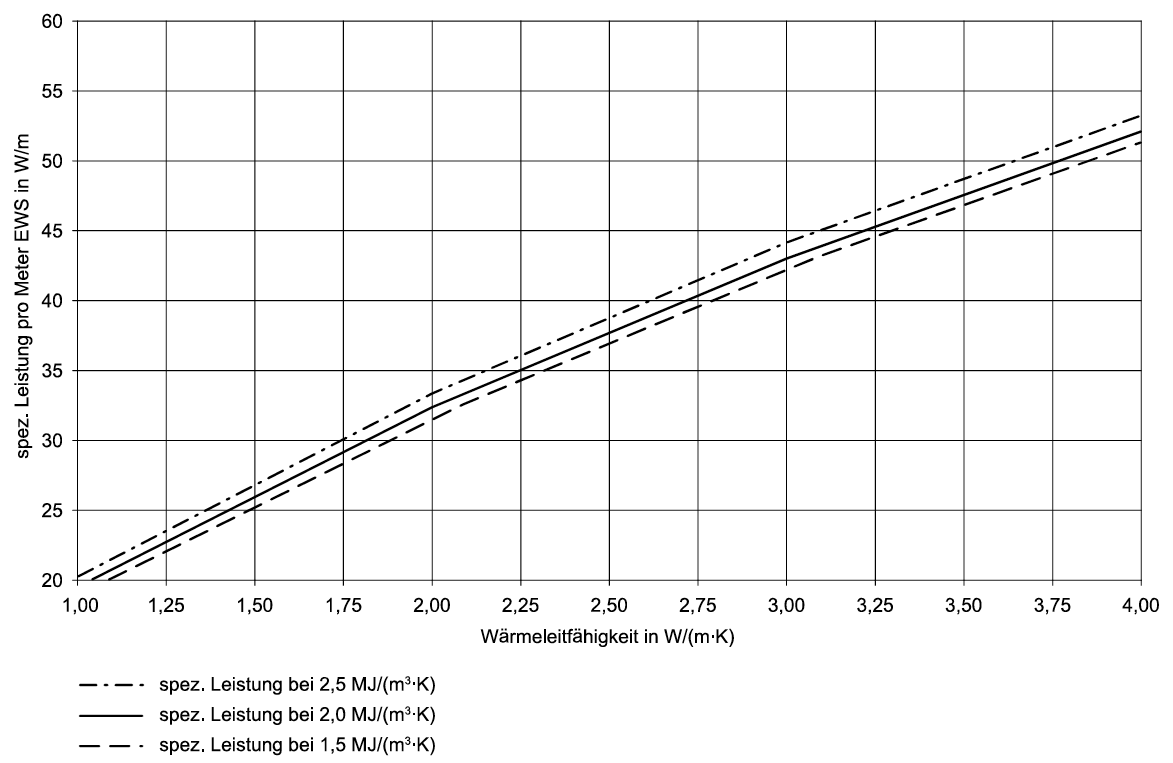
\includegraphics[width=.96\linewidth]{Figs/q_max_norm.png}  
\end{subfigure}
\begin{subfigure}{.48\textwidth}
  \centering
  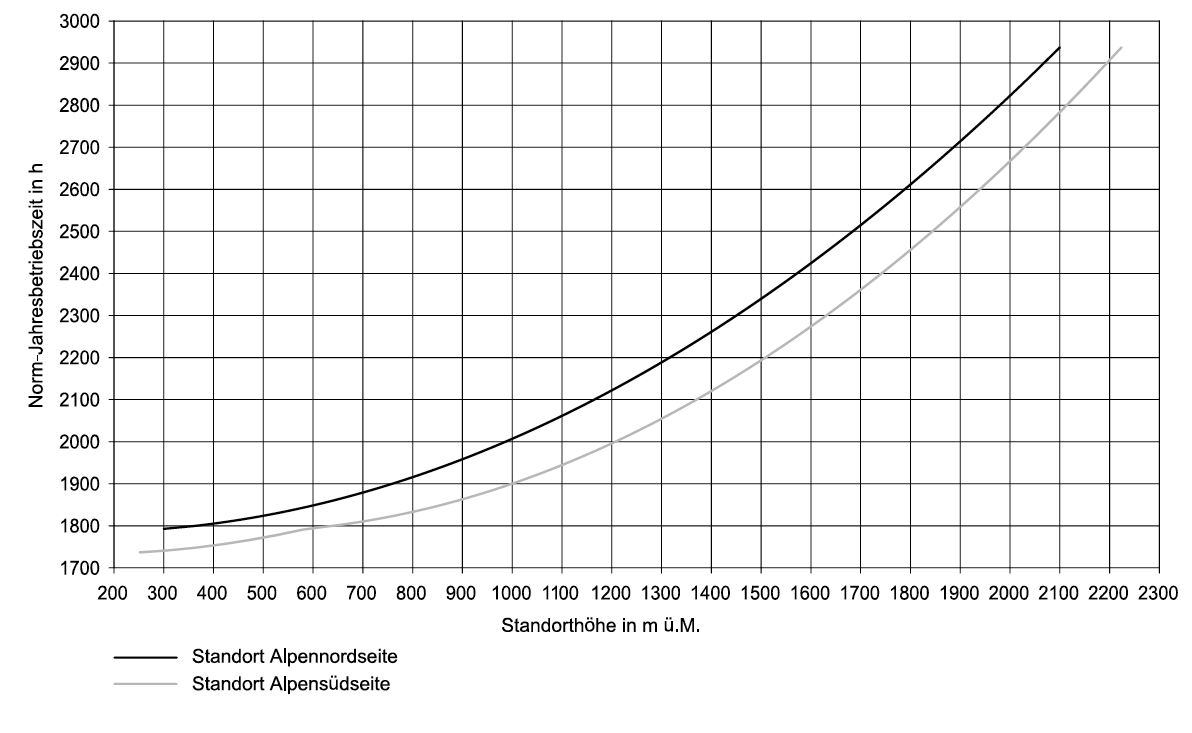
\includegraphics[width=\linewidth]{Figs/t_op_norm.png}  
\end{subfigure}
\caption{a) nominal heat extraction rate ($q_{max}$) for a duplex BHE (32mm) at $H=100m$, $T_g=10$, $t_op = 1850h$ as a function of $\lambda$ and $\rho C$, b) nominal operating time ($t_{op}$) as a function of altitude north and south of the alps \citep{sia_sondes_2010} (Fig. 7 \& 10).}
\label{fig:t_q_norm}
\end{figure}

\subsection{Temperature profile of a BHE installation}
\label{model_intro}

To quantify the temperature field of a BHE, we distinguish between the processes inside and outside the BHE. The temperature drop inside the BHE, i.e. between the heat carrier fluid at mean temperature $T_f$ and the borehole wall at temperature $T_b$, is a function of the heat extraction rate and the effective thermal resistance of the boorehole, such that \citep{claesson_conductive_1988}:

\begin{equation}
\label{eq:T_b}
    T_b(t) - T_f(t) = q_{max}*R_b^*
\end{equation}

The inlet temperature of the fluid may be obtained from the following equation \citep{pahud_geothermal_2002}, p. 43:

\begin{equation}
    q_{max} * H = \dot{m} * cp_f * (T_{f, out} - T_{f, in})
\end{equation}

where $Q_{HP}$ is the heat extraction power of the heat pump, $\dot{m}$ is the mass flow rate of the fluid (in $kg/s$), $cp_{f}$ is the thermal capacity of the fluid (in $J/kgK$) and $T_{f,in}$ and $T_{f,out}$ are the inlet and outlet temperatures.

The temperature at the borehole wall $T_b$ differs from the undisturbed ground temperature $T_g$ by a temperature drop $\Delta T_b$. It varies with depth ($z$), so the average value along the borehole may be obtained by numerical integration ($z = \overline{z}$) or, in a simplified way, by taking $z = H/2$. The borehole wall temperature $T_b$, with $r = r_b$, is hence computed as:
\begin{equation}
    T_b(z, t) = T_g(z) - \Delta T_b(z, t)
\end{equation}

\begin{figure}
    \centering
    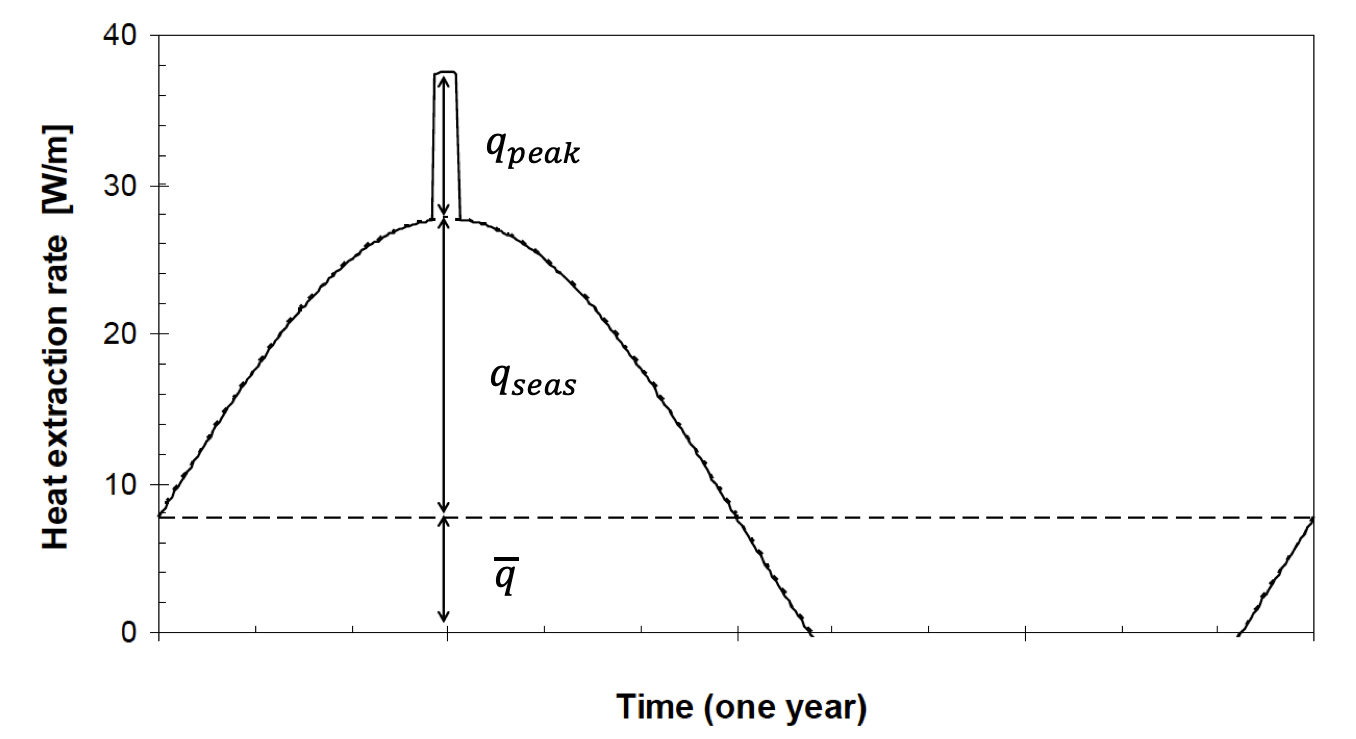
\includegraphics[width=.6\linewidth]{Figs/q_seasonal.png}
    \caption{"Simplified heat extraction rate evolution for a typical year (constant + periodic + pulse)" \citep{pahud_geothermal_2002}.}
    \label{fig:q_seasonal}
\end{figure}

The $\Delta T_b(z, t)$ is characterized by a long-term (\textit{LT}), seasonal (\textit{seas}) and short-term (\textit{peak}) component. To perform system sizing based on the minimum fluid temperature condition, all three effects have to be taken into account to give a "worst-case" scenario. A method to model these effects, shown in Fig.~\ref{fig:q_seasonal}, is suggested in \citep{claesson_conductive_1988} and summarized in \citep{pahud_geothermal_2002}, p.43. Long-term effects are represented by a constant heat extraction rate $\overline{q}$, which is typically assessed for a planning horizon ($t_{dim}$) of 50 years. Seasonal effects are represented as a sinusoidal heat extraction with peak rate $q_{seas}$ and period 1 year, so that the annual integral is zero. The peak extraction, which occurs at maximum seasonal extraction, has a duration $t_{peak}$ (typically 1-10 days). The energy extracted from this pulse is neglected. To obtain $\Delta T_b$, each heat extraction rate is multiplied with a respective thermal resistance ($R_{LT},R_{seas},R_{peak}$):

\begin{equation}
\label{eq:dT_b}
    \textstyle \Delta T_b(z, t) = \overline{q} * R_{LT}(z, t) + q_{seas} * R_{seas, max} + q_{peak} * R_{peak}(t)
\end{equation}
where
\begin{equation*}
    \overline{q} = \frac{t_{op}}{365*24} * q_{max}, \quad q_{seas} = 0.5 * q_{max}, \quad q_{peak} = q_{max} - \overline{q} - q_{seas}
\end{equation*}

A combination of Eqs.~\ref{eq:T_b}-\ref{eq:dT_b} gives the following technical condition to be fulfilled:

\begin{equation}
    \textstyle T_g(\frac{H}{2}) - \overline{q} * R_{LT}(\overline{z}, t_{dim}) - q_{seas} * R_{seas, max} - q_{peak} * R_{peak}(t_{peak}) - q_{max}*R_b^* \geq T_{f, min}
\end{equation}

The seasonal and peak effects are of a short duration, and can be approximated as functions of the technical and physical parameters only (i.e. $r_b, \lambda, \alpha$). Their penetration radius is a few meters and lies below the minimum borehole distance $B_{min} = 5m$, so seasonal and peak effects of neighboring boreholes do not interfere with each other. Consequently, $R_{seas}$ and $R_{peak}$ are "quasi-constants" in the large-scale geothermal potential estimation. The analytic formulas for both components are given in Section~\ref{seas_peak}. 

The long-term temperature drop, however, may have an impact on surrounding boreholes. Fig.~\ref{fig:T_field} shows the long-term $\Delta T$ for different times, a) at the borehole wall as a function of $z$ and b) integrated along $z$ (denoted as $\overline{z}$) as a function of distance to the borehole. Most of the temperature drop occurs during the first 10 years of operation, while the temperature drop after the planning horizon of 50 years is small. 
Figure~\ref{fig:T_field}a shows that the approximation of $z=H/2$ quantifies the worst-case temperature drop along the borehole. The rules of thumb given in \citep{pahud_geothermal_2002}, p. 50, state that the temperature drop is small at a horizontal distance of $r>H/2$ from the center of the BHE, and negligible for $r>H$. This is confirmed by Fig.~\ref{fig:T_field}b. 
We refer to the long-term temperature drop as $\Delta T_{LT}$ and include $r$ as variable, as also distances $r>r_b$ are of interest:

\begin{equation}
    \Delta T_{LT}(r, z, t) = \overline{q} * R_{LT}(r, z, t)
\end{equation}

\begin{figure}
    \centering
    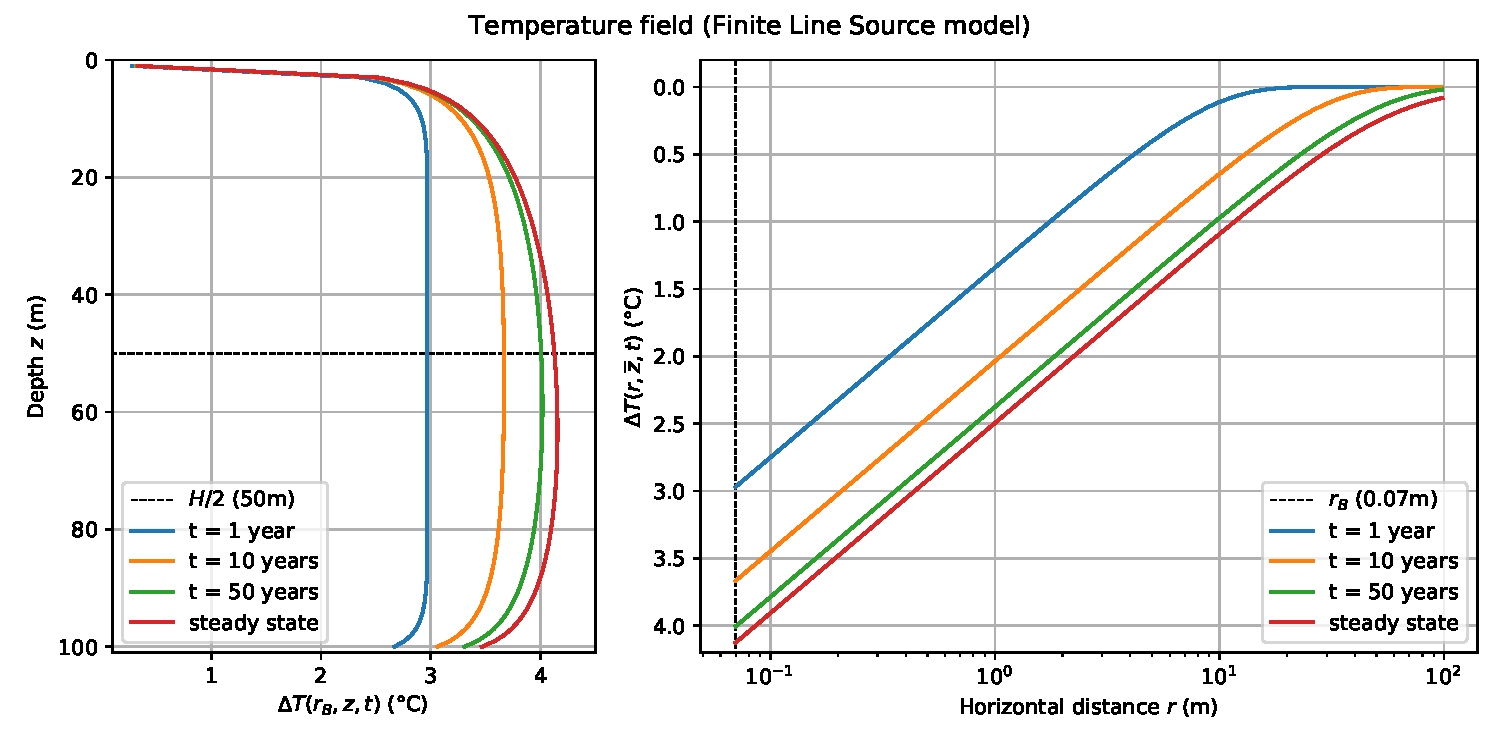
\includegraphics[width=.9\linewidth]{Figs/temp_field_FLS.pdf}
    \caption{a) Long-term variation of the ground temperature at the borehole wall ($\Delta T_{LT}(r_b, z, t)$) as a function of depth ($z$), b) Long-term temperature variation integrated along $z$ ($\Delta T_{LT}(r, \overline{z}, t)$) as a function of distance to the BHE ($r$).}
    \label{fig:T_field}
\end{figure}

\subsection{Analytic models and approximations}

According to \citet{claesson_conductive_1988}, the heat transfer of a BHE can be modelled with good accuracy as a purely conductive process in a homogeneous medium. This means that convective heat transfers are negligible. Furthermore, the thermal conductivity $\lambda$ of stratified ground with multiple layers may be approximated as a weighted average of the properties of the layers. 
\citet{claesson_conductive_1988} also argue that the undisturbed ground temperature $T_g(z)$ along the borehole can be approximated without loss of accuracy by the undisturbed ground temperature at half the borehole height, i.e. $T_g(\overline{z}) \approx T_g(H/2)$. 

The thermal resistance ($R$) is represented in a general form through so-called \textit{g-functions}. They are are dimensionless step-response functions characterizing the thermodynamic behaviour of the ground:

\begin{equation}
    R = \frac{1}{2 \pi \lambda} \, \mathrm{g}\left( \frac{t}{t_s}, \frac{r}{H} \right), \quad \frac{t}{t_s} > 0
\end{equation}

The g-function is a function of the ratio between the time $t$ and the BHE's time constant $t_s$, as well as the ratio between the horizontal distance to the BHE center $r$ ($r_b$ for a single borehole) and the borehole length $H$. The ratio $t/t_s$ may also be referred to as Eskilson's number (Es) \citep{pahud_geothermal_2002}. For simplicity, only the variables (i.e. $r, z, t$, not the parameters $t_s, H$) are indicated in the argument of the g-function (where relevant). The time constant $t_s$, typically between $35-140a$, is defined as:

\begin{equation}
    t_s = \frac{H^2}{9 \alpha}
\end{equation}

The steady state is reached when $\ln{(t/t_s)} = 2$, i.e. $t_{ss} = e^2 t_s \approx 7.5 t_s$ \citep{wagner_erdsondenpotenzial_2014}. 

\textbf{Finite Line Source (FLS)}. 
The FLS describes the most accurate analytic model used in the literature. It is a solution to the heat conduction equation that satisfies the boundary conditions $T(r, z=0, t=0) = 0$. The g-function of the transient solution is given by \citep{pahud_geothermal_2002}:

\begin{equation}
\label{eq:FLS}
    \mathrm{g}_{FLS}(r, z, t) = \frac{1}{2} \int_{D}^{D+H} \left( \frac{1}{r_+} \mathrm{erfc}\left(\frac{r_+}{\sqrt{4 \alpha t}}\right) - \frac{1}{r_-}\mathrm{erfc}\left(\frac{r_-}{\sqrt{4 \alpha t}}\right) \right) ds
\end{equation}

where
\begin{equation*}
    r_+ = \sqrt{r^2 + (z - s)^2}, \quad r_- = \sqrt{r^2 + (z + s)^2}
\end{equation*}

\begin{equation*}
   \mathrm{erfc}(x) = \frac{2}{\sqrt{\pi}} \int_{x}^{\infty} e^{-\mu^2} d\mu
\end{equation*}

The steady-state solution (valid for $t > t_{ss}$) is defined as:

\begin{equation}
\label{eq:FLS_ss}
    \mathrm{g}_{FLS,ss}(r, z) = \frac{1}{2} \int_{D}^{D+H} \left( \frac{1}{r_+} - \frac{1}{r_-} \right) ds
\end{equation}

For many borehole applications, the mean temperature along the borehole length is of interest. This can be obtained by integrating $\mathrm{g}_{FLS}(r, z, t) $ along the $z$-axis. \citet{claesson_analytical_2011} provide the following analytical solution for this integration, which is very computationally efficient: 

\begin{equation}
\label{eq:FLS_int}
    \mathrm{g}_{FLS}(r, \overline{z}, t) = \frac{1}{2} \int_{\frac{1}{\sqrt{4 \alpha t}}}^{\infty}  e^{- r^2 s^2} \ \frac{I_{ls}(Hs, Ds)}{H s^2} \ ds
\end{equation}

where
\begin{equation*}
    I_{ls}(h, d) = 2\ \mathrm{ierf}(h) + 2\ \mathrm{ierf}(h + 2d) - \mathrm{ierf}(2h + 2d) - \mathrm{ierf}(2d)
\end{equation*}

\begin{equation*}
    \mathrm{ierf}(x) = \int_0^x \mathrm{erf}(u) du 
                     = x \ \mathrm{erf}(x) - \frac{1}{\sqrt{\pi}} (1 - e^{-x^2})
    \qquad
    \mathrm{erf}(x) = \frac{2}{\sqrt{\pi}} \int_0^x e^{-\mu^2} d \mu 
\end{equation*}

The FLS can be simplified under certain assumptions by simpler models, namely the infinite line source model (ILS) and an asymptotic approximation of the FLS model, here referred to as Eskilson's approximation (Esk). A comparison of all methods is provided in Section~\ref{comparison}.
\\

\textbf{Infinite Line Source (ILS)}. The ILS approximation is defined as \citep{poppel_grenzabstande_2017}:

\begin{equation}
\label{eq:ILS}
    \mathrm{g}_{ILS}(r, t) = \frac{1}{2} \int_\frac{r^2}{4 \alpha t}^\infty \frac{e^{-u}}{u}du 
                  = \frac{1}{2} E_1\left(\frac{r^2}{4 \alpha t}\right)
\end{equation}

The error between the ILS and FLS is negligible for $t < 0.1 t_s$ \citep{claesson_conductive_1988}, making it particularly suitable for short and medium-term analyses. For $t<t_s$, it is accurate with a bounded error (see \ref{comparison}), but as it does not reach a steady state (due to the assumed infinite length), it is not suitable for modelling ground temperature at $t>t_s$.
\\

\textbf{Eskilson's approximation (Esk)}.
\citet{eskilson_thermal_1987} proposes to model the temperature drop along the borehole as a function of the two asymptotes of the FLS model. The lower asymptote is valid for $t < t_s$ and represents the transient behaviour ($\mathrm{g}_{Esk, trans}$). For $t > t_s$, the upper asymptote represents the (quasi) steady-state ($\mathrm{g}_{Esk, qss}$). The g-function of the asymptotic approximation is hence defined as:

\begin{equation}
    g_{Esk}(r, t) = \left\{
        \begin{matrix}
            \mathrm{g}_{Esk, trans} & t_{min} < t < t_s   \\ 
            \mathrm{g}_{Esk, qss}    & t > t_s           
        \end{matrix} 
\right.
\end{equation}

The \textit{transient asymptote} is an approximation of the ILS \citep{wagner_erdwarmesonden._2019}. Two equivalent formulations of $\mathrm{g}_{Esk, trans}$ exist. The first is derived from the mathematical approximation of the exponential integral $E_1$ in Eq.~\ref{eq:ILS}, while the second represents the physical process. The expressions are \citep{pahud_geothermal_2002}: 

\begin{equation}
\label{eq:Esk_trans}
    \mathrm{g}_{Esk, trans}(r, t) = \frac{1}{2} \left(\ln\left(\frac{4 \alpha t}{r^2}\right) - \gamma\right)
                                  = \ln\left(\frac{H}{2 r}\right) + \frac{1}{2} \ln\left(\frac{t}{t_s}\right), \quad
    t_{min} < t < t_s
\end{equation}

While the second expression is more intuitive, the first provides more information on the validity of the approach. It is derived from the following approximation of the exponential integral:

\begin{equation}
\label{eq:apx}
    E_1\left(x\right) \approx \ln\left(\frac{1}{x}\right) - \gamma, \quad x \ll 1
\end{equation}

where $\gamma$ is Euler's constant (0.57221...). To obtain Eq.~\ref{eq:Esk_trans}, we substitute Eq.~\ref{eq:apx} in Eq.~\ref{eq:ILS}.
Equation~\ref{eq:apx} approximates the ILS for all $x < 0.05$ with negligible error. For $x = r^2/(4 \alpha t)$ and $r = r_b$ (the borehole wall), this gives a minimum time for the transient asymptote of:

\begin{equation}
    t_{min} = \frac{5 r_b^2}{\alpha}, \quad r_b \ll H
\end{equation}

The values of $t_{min}$ typically lie below $6h$, so the condition is fulfilled for all timescales of interest.

If the temperature at larger distances from the borehole is of interest ($r \gg r_b$), for example for modelling borehole fields, the condition for the validity of Eq.~\ref{eq:Esk_trans} becomes:

\begin{equation}
\label{eq:r_cond}
    r < \sqrt{(0.2 \alpha t )}
\end{equation}

The interaction between boreholes is only of interest in the long term. On this temporal scale, we obtain $r_{dim} < 18m$ for the planning horizon of 50 years, $r_{qss} < 0.15H$ for $t_s$ and $r_{ss} < 0.4H$ for $t_{ss}$.

The \textit{steady-state asymptote} approximates the steady-state solution of the FLS (Eq.~\ref{eq:FLS_ss}). We refer to it as \textit{quasi steady-state}. According to \citet{eskilson_thermal_1987}, the quasi steady-state is given by:

\begin{equation}
\label{eq:Esk_qss}
    \mathrm{g}_{Esk, qss}(r) = \ln\left(\frac{H}{2 r}\right), \quad t > t_s
\end{equation}

From Eqs.~\ref{eq:Esk_trans} and \ref{eq:Esk_qss} it is easy to see that the two asymptotes intersect at $t = t_s$.
As the Esk model is practically equivalent to the ILS solution for $t_{min} < t < t_s$ (provided Eq.~\ref{eq:r_cond} is fulfilled), the transient asymptote has a negligible error with respect to the FLS for $t < 0.1 t_s$, and a bounded error for $t = t_s$. The transient asymptote also has a bounded error with respect to the FLS.

\subsubsection{Model comparison}
\label{comparison}

\begin{figure}[t]
    \centering
    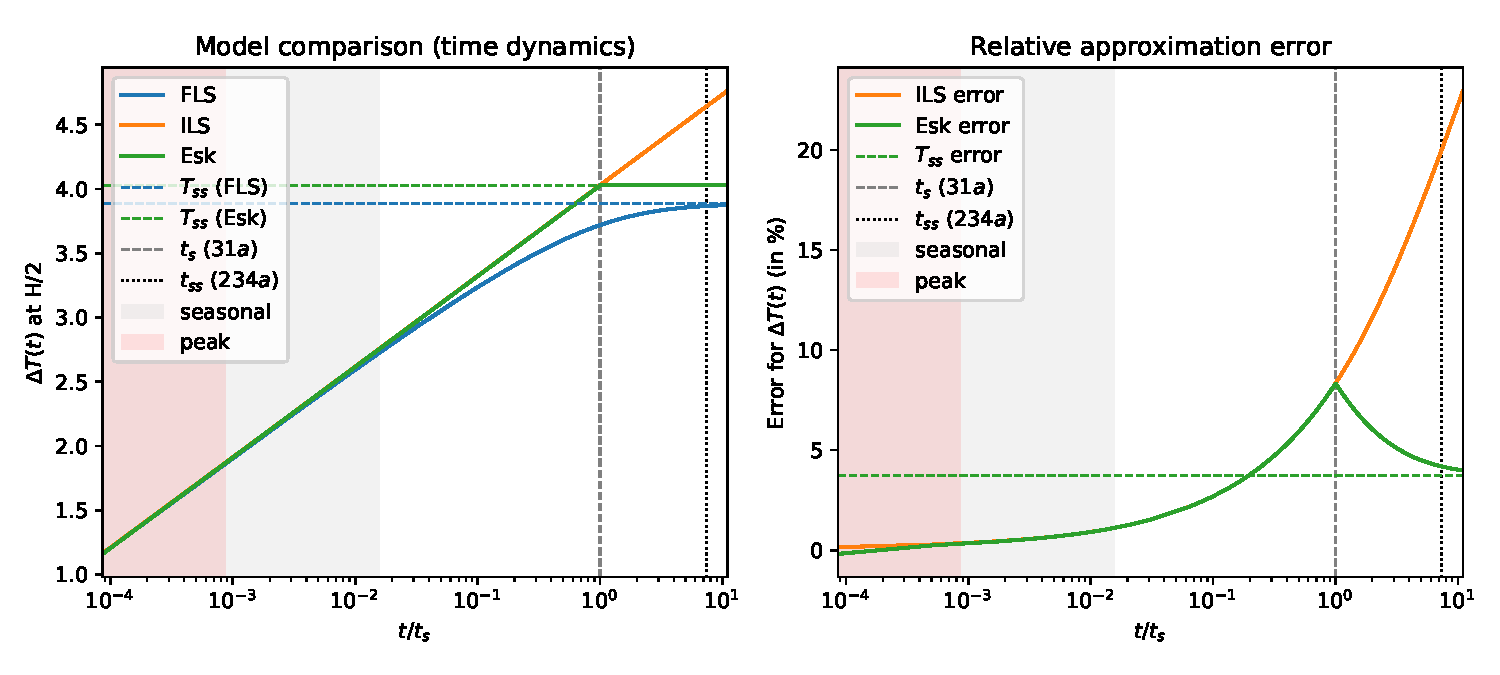
\includegraphics[width=.9\linewidth]{Figs/FLS_ILS_Esk_compare_ts.pdf}
    \caption{a) Temporal dynamics of the temperature variation along the borehole (shape of the "g-function") for the Finite Line Source (FLS), Infinite Line Source (ILS) and asymptotic (Esk) models, b) relative error for the temperature variation, as percentage of the $\Delta T_{FLS}$. The time duration of peak (red) and seasonal (grey) effects are highlighted.}
    \label{fig:T_dynamics}
\end{figure}

As mentioned above, the approximations of the FLS model are valid under certain assumptions, but may significantly speed-up the modelling time (even though the formulation in Eq.~\ref{eq:FLS_int} is already much faster than Eq.~\ref{eq:FLS}). To understand the ranges of validity and the error induced by the use of the approximations, we compare the different models for different time scales and distances to the borehole. All examples are shown for a borehole of 100m length, but the patterns are nearly identical for longer BHE's. In general, the temperature drop ($\Delta T$) along the borehole is smaller for larger $H$, hence leading to smaller absolute, but similar relative errors. 

Figure~\ref{fig:T_dynamics} shows a comparison between the models for different time scales at the borehole wall ($r = r_b$). We can see that for short time scales (red/grey), all models have a negligible error (up to $1\%$). 
Hence, any approximation may be used to model both peak and seasonal effects. At larger time scales, the ILS model starts to diverge from the FLS solution. 
This is expected, as the ILS never reaches a steady-state due to its infinite length. In this context, \citet{bandos_finite_2009} provide a formulation for a semi-infinite line source (SILS), which does reach a steady state. 

The Esk model is quasi-equivalent to the ILS for $t_{min} < t < t_s$, and reaches its steady-state for $t > t_s$. The figure shows that the upper asymptote overestimates the steady-state temperature by $3.7\%$, with the largest error occurring around $t = t_s$ ($\approx 8\%$). These percentages are valid for all borehole lengths. 
For typical boreholes of $H=100-200m$, the time scales with the maximum error (around $t_s$) correspond to the time scales of highest interest. 
As the absolute difference is relatively small, this may not have a large impact for modelling individual boreholes, and the asymptotic steady-state $\mathrm{g}_{Esk, qss}$ can be safely used. For modelling large borehole fields, however, the error accumulates, which can lead to significant differences in the estimated potential. For large-scale studies, the exact FLS solution should hence be used.

\begin{figure}[t]
    \centering
    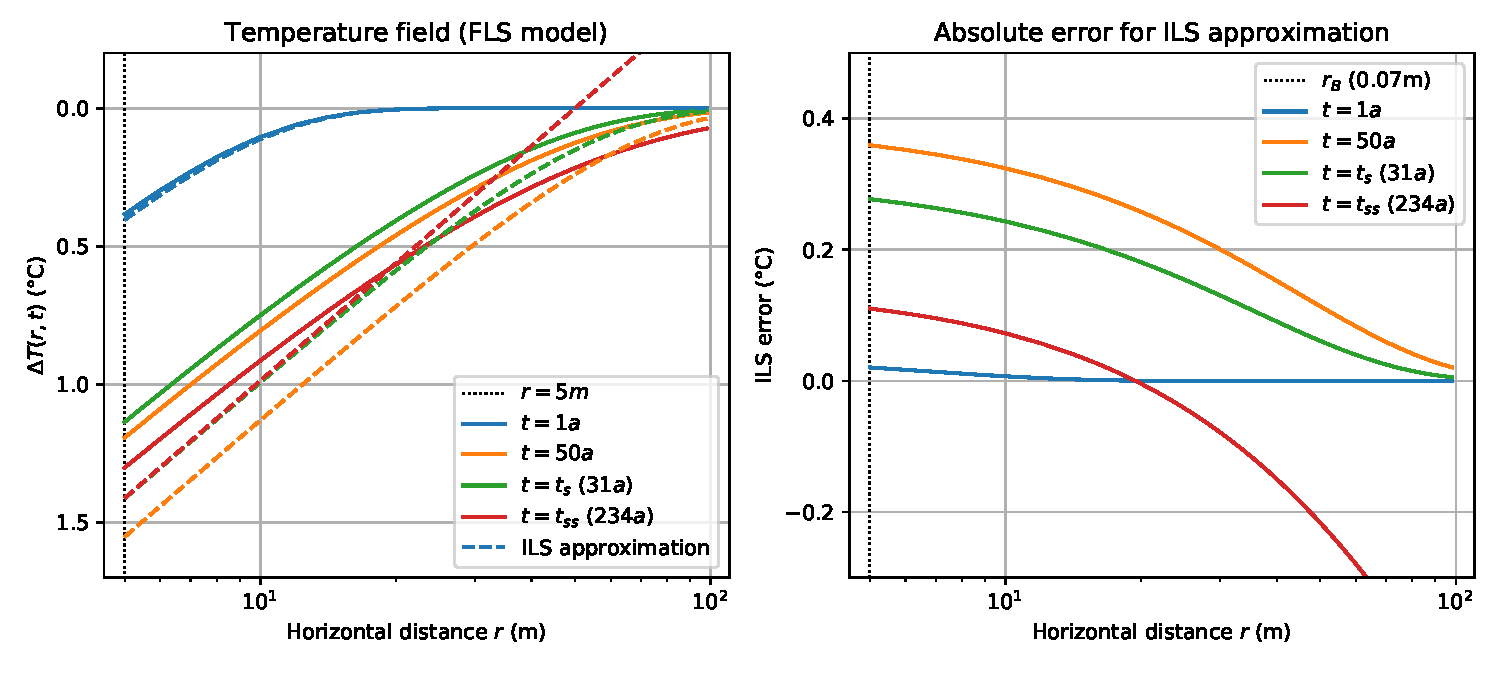
\includegraphics[width=.9\linewidth]{Figs/FLS_ILS_compare_r.pdf}
    \caption{a) Temperature field with distance to the BHE (length 100m) on logarithmic scale. The Infinite Line Source (with $\mathrm{g}_{Esk, qss}$ for $t = t_{ss}$) is shown for comparison (dashed lines). b) Absolute error (in $\circ$C) for the ILS model. The example shows a BHE of 100m length.}
    \label{fig:r_field}
\end{figure}

To assess the effect of adjacent boreholes, the temperature fields at large distances from the borehole ($5m < r < H$) are of interest. As seasonal and peak effects have a penetration depth that is lower than the minimum borehole distance of $5m$, only long-term effects are relevant. Figure~\ref{fig:r_field} shows the temperature drop in the ground for three long-term time intervals: the typical planning horizon ($t_{dim}$) for BHEs of 50 years, the quasi-steady-state $t_s$, where the temperature drop has reached around $95\%$ of its final value, and the actual steady state ($t_{ss}$). For comparison, also a short horizon of 1 year is shown.

While the temperature drop increases logarithmically for small distances, it trails off for distances that approach the borehole length $H$. In this range, Eq.~\ref{eq:apx} is no longer valid, so the transient asymptote cannot be used. This can be seen by the unrealistic steady-state solution, which represents the Esk steady-state asymptote (see Eq.~\ref{eq:Esk_qss}). It reaches a value of $0$ at $H/2$ and has negative values after, which is infeasible.

As Fig.~\ref{fig:T_dynamics} suggests, the error between the ILS and the FLS model increases with time, up to $0.1-0.3 ^\circ$C for the radii of interest. While this may  be negligible for a single neighbor, the error accumulates for borehole fields.  The exact FLS solution should hence be used for modelling large-scale geothermal potentials.

\subsection{Short-term, seasonal and long-term effects}
\label{seas_peak}

As it was shown in Fig.~\ref{fig:q_seasonal}, the minimum temperature at the borehole wall consists of a long-term, a seasonal and a peak component, each obtained by multiplying the respective heat extraction rate ($\overline{q}, q_{seas}, q_{peak}$) with its thermal resistance ($R_{LT},R_{seas},R_{peak}$, see Eq.~\ref{eq:dT_b}). 

\textbf{Long-term effects} may be assessed at $t = t_{dim}$ (typically 50 years), at quasi steady-state ($t = t_s$) or at steady state ($t = t_{ss}$). It is common to use the quasi steady-state asymptote for a conservative approximation of a \textit{single borehole}, as it overestimates the maximum temperature drop (see Fig.~\ref{fig:T_dynamics}). Examples for this approach are \cite{claesson_conductive_1988} and \cite{pahud_geothermal_2002}. 

For \textbf{multiple boreholes}, the g-functions of each borehole are superposed. As we saw in Section \ref{comparison}, only the exact FLS is appropriate for a realistic superposition of multiple BHEs, as an accumulation of the error should be avoided.
The formula for the long-term resistance of borehole $i$ in a field of $N$ boreholes then becomes (adapted from \cite{claesson_analytical_2011}):

\begin{equation}
    R_{LT, i}(t_{dim}) = \frac{1}{2 \pi \lambda} \mathrm{g}_{Esk, qss}(r_b) + \frac{1}{2 \pi \lambda} \sum_{j=1}^N \mathrm{g}_{FLS}(r_{i,j}, \overline{z}, t_{dim}) ,
    \quad i,j = 1, 2, ..., N
\end{equation}

where $i \neq j$ and $\mathrm{g}(r, \overline{z}, t)$ is the FLS solution integrated along the borehole length ($\overline{z}$). If a single borehole is considered, only the first term of the addition is relevant.

\textbf{Seasonal effects} are modelled as a periodic heat extraction. Effects from neighboring boreholes can be ignored if the minimum spacing ($B_{min}$) fulfills the following condition:

\begin{equation}
    B_{min} > 0.7 \sqrt{\alpha t_{seas}}
\end{equation}

As the minimum spacing is set to $5m$ \cite{sia_sondes_2010}, this criterion is fulfilled for the period of the seasonal variation ($t_{seas} = 1a$). The thermal diffusivities in Switzerland (see Table~\ref{tab:phys_params}) result in $B_{min} \approx 3.5-4.5m$. The maximum periodic thermal resistance is given by \citep{claesson_conductive_1988, pahud_geothermal_2002}:

\begin{equation}
    R_{seas, max} = \frac{1}{2 \pi \lambda} \sqrt{\left(\ln(2/r_{pb}^\prime \right) - \gamma)^2 + \pi^2/16}
\end{equation}

where
\begin{equation*}
    r_{pb}^\prime = r_b \sqrt{2}/\delta < 0.1, \quad \delta = \sqrt{ \alpha t_{seas} / \pi}
\end{equation*}
    
The penetration depth of the temperature drop is denoted as $\delta$, which is around $3-4m$ for Switzerland. Seasonal effects hence do not impact adjacent boreholes. 

\textbf{Short-term effects} are represented by a heat extraction pulse at $q_{max}$ for a duration $t_{peak}$, typically 1-10 days (see Table~\ref{tab:tech_design_params}). Due to the short duration of the pulse, the asymptotic transient approximation is valid with negligible error. Thermal effects have an even smaller penetration depth than seasonal effects, so no surrounding boreholes need to be considered. The thermal resistance can hence be obtained as:

\begin{equation}
    \mathrm{R}_{peak}(t_{peak}) = \frac{1}{2 \pi \lambda} \ \mathrm{g}_{Esk, trans}(r_b, t_{peak})
\end{equation}


%\section{Hybrid system optimization}
